
\chapter{Method 1: Direct intersection}
\label{ch:direct_intersection}

The first presented method to extract a triangulated surface from the VML's data model is by directly processing the stored triangles inside the VML's regular grid.
This approach is the most naive, computationally intensive, but, in theory, most accurate.
It is conceptually equivalent to directly intersecting the mesh of the stock with each swept volume mesh.
Boolean operations on triangle meshes are already available in most CAD kernels.
However, these kernels usually require the meshes to be closed.
Due to the triangle elimination strategy using cell classification, \cf section \ref{sec:classification}, the meshes stored in the regular grid are no longer closed.
Thus, regular CAD kernels cannot be used to intersect the meshes maintained by the VML and a custom mesh intersection algorithm has been developed.
The idea of this approach is based on a paper about finding and deforming the intersection between two meshes as well as applying textures to those regions to increase the realism in computer graphics, \ie computer games \cite{mesh_intersection}.

\section{Concept}
\label{sec:direct_intersection_concept}

Every time a swept volume is added to the VML, a unique id is generated and assigned to each of the swept volume's triangles before they are mapped to the cells of the regular grid.
As the stock is internally treated as a swept volume, by inverting the surface normals, all stock triangles are also assigned a unique id.
These ids allow to separate the triangles contained in the regular grid into the previous swept volumes, referred to as structures.
The separated structures are processed in pairs.
Each pair is united into a new structure.
The union of the two structure meshes is calculated by intersecting each triangle of one mesh with each triangle of the other mesh.
If two triangles intersect, the intersection line is recorded for both triangles.
After intersection, each triangle with intersection lines is split along these lines, retriangulated and replaced by the triangles resulting from the retriangulation.
All previous intersection lines are now edges of new triangles.
Each triangle of one structure is then tested against the other structure, whether the triangle is inside or outside the other structure, \eg by casting a ray from the triangle to the other structure.
As all triangles intersecting the opposite structure have been split, this property should be unambiguously determinable for each triangle.
By removing all triangles inside the opposite structure, the remaining triangles form a new surface which corresponds to the union of both structures.
This new structure is then again pairwise united with other structures until only one structure is left, \ie all structures are reduced to one.
This final structure is the reconstructed surface of the VML's data model.
Figure \ref{fig:cube2} demonstrates this workflow by the example of intersecting a cube with a cuboid.

\begin{figure}
	\centering
	\begin{subfigure}[t]{0.3\textwidth}
		\centering
		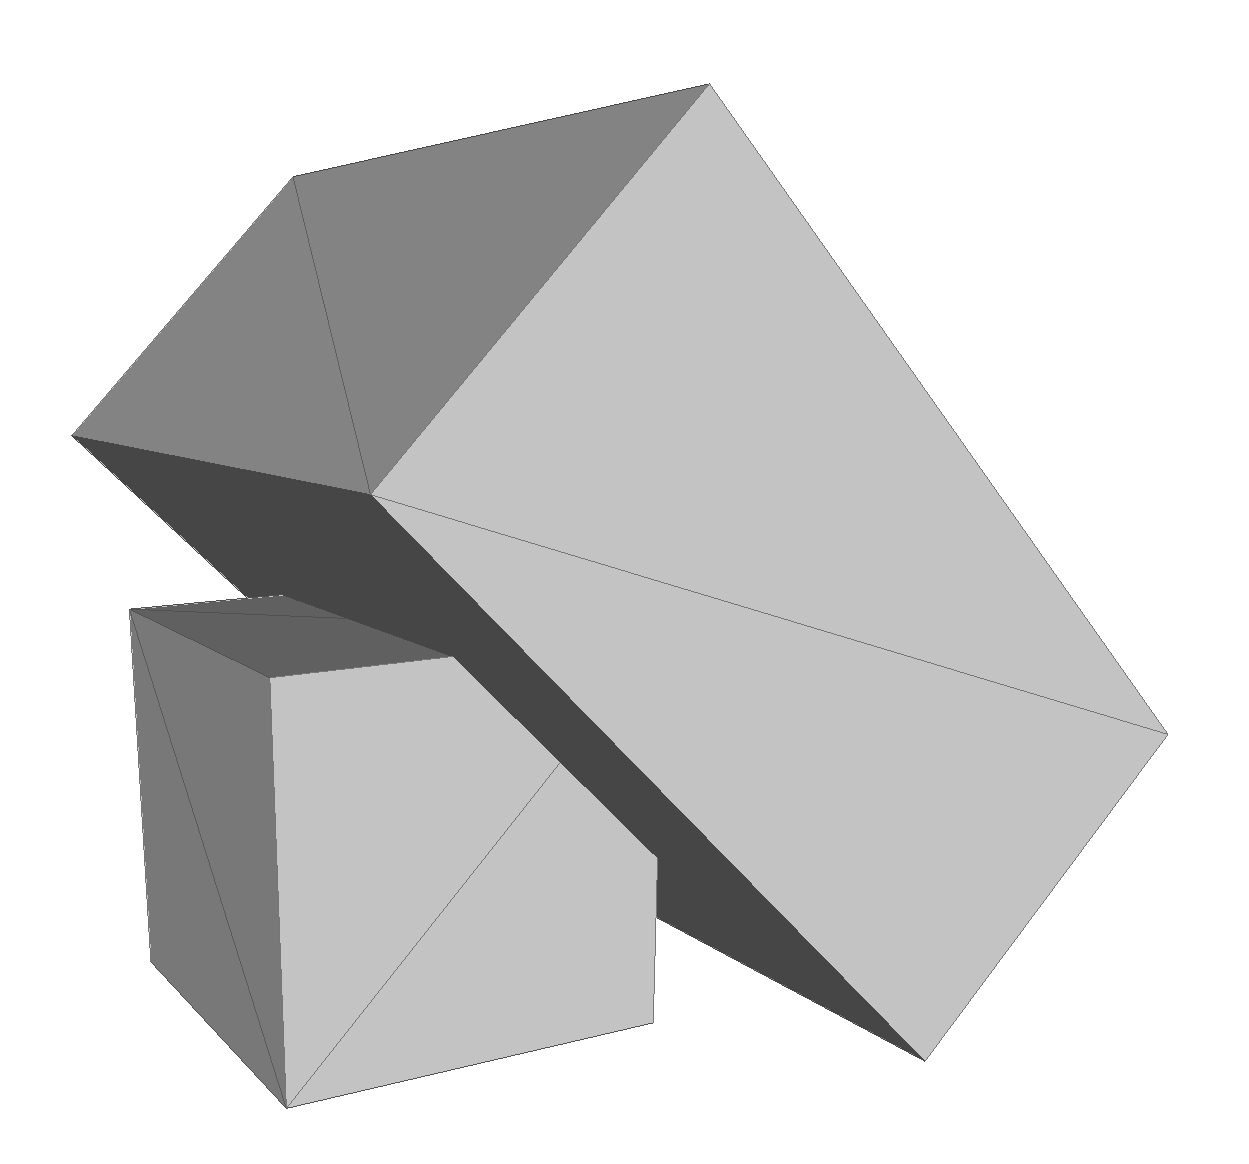
\includegraphics[width=\textwidth]{images/cube2_stock_sv}
		\caption{Stock and SV}
		\label{fig:cube2_stock_sv}
	\end{subfigure}
	\begin{subfigure}[t]{0.3\textwidth}
		\centering
		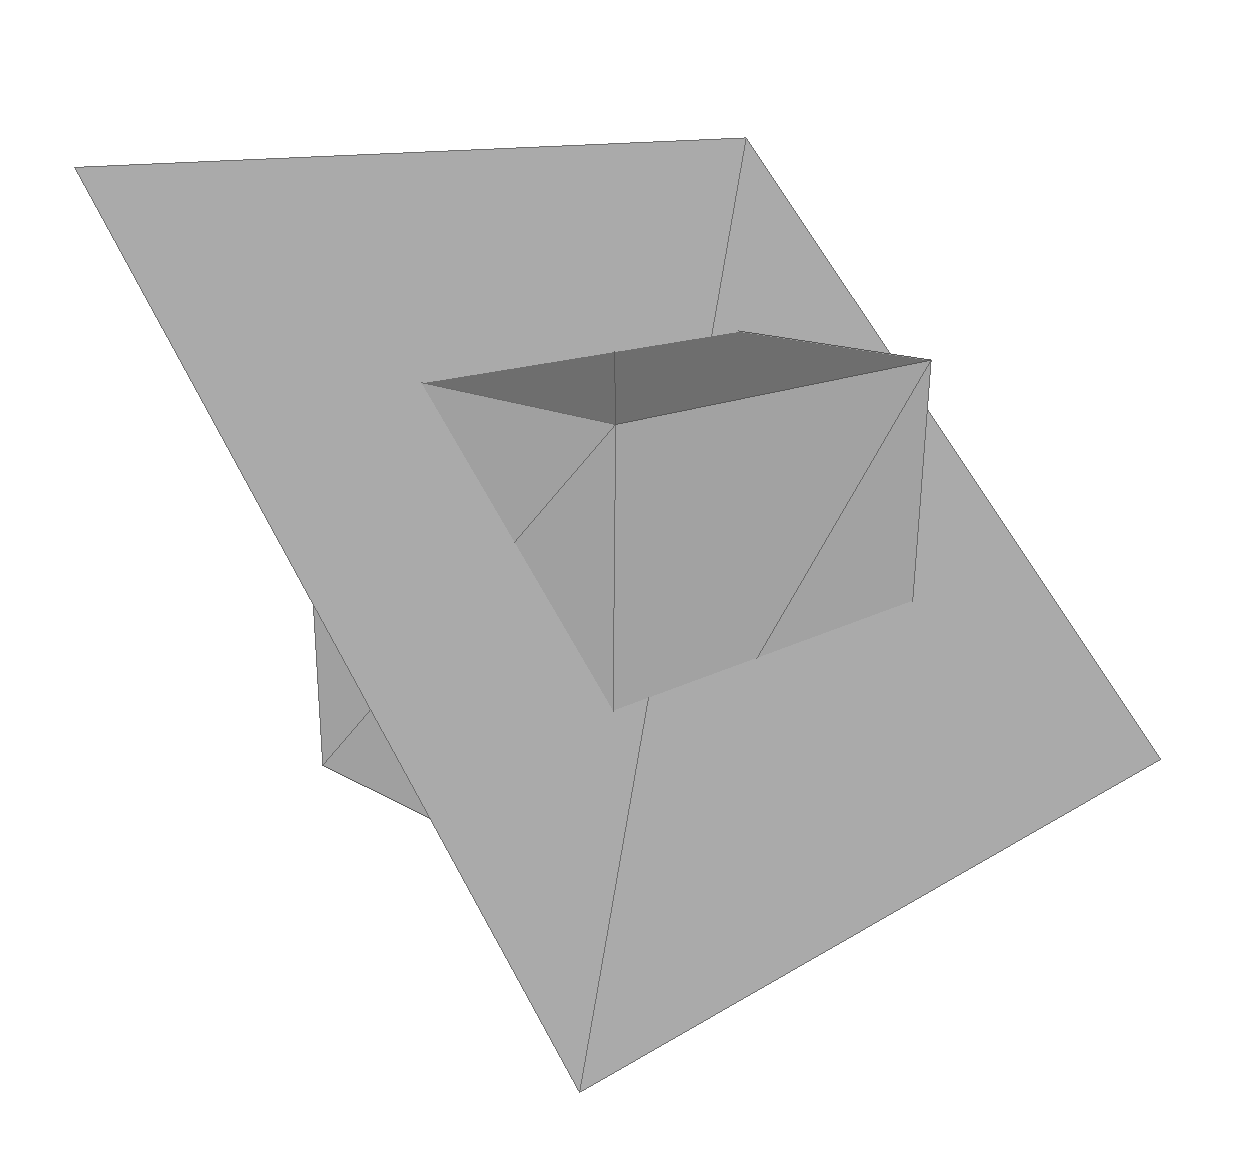
\includegraphics[width=\textwidth]{images/cube2_classified}
		\caption{VML}
		\label{fig:cube2_classified}
	\end{subfigure}
	\begin{subfigure}[t]{0.3\textwidth}
		\centering
		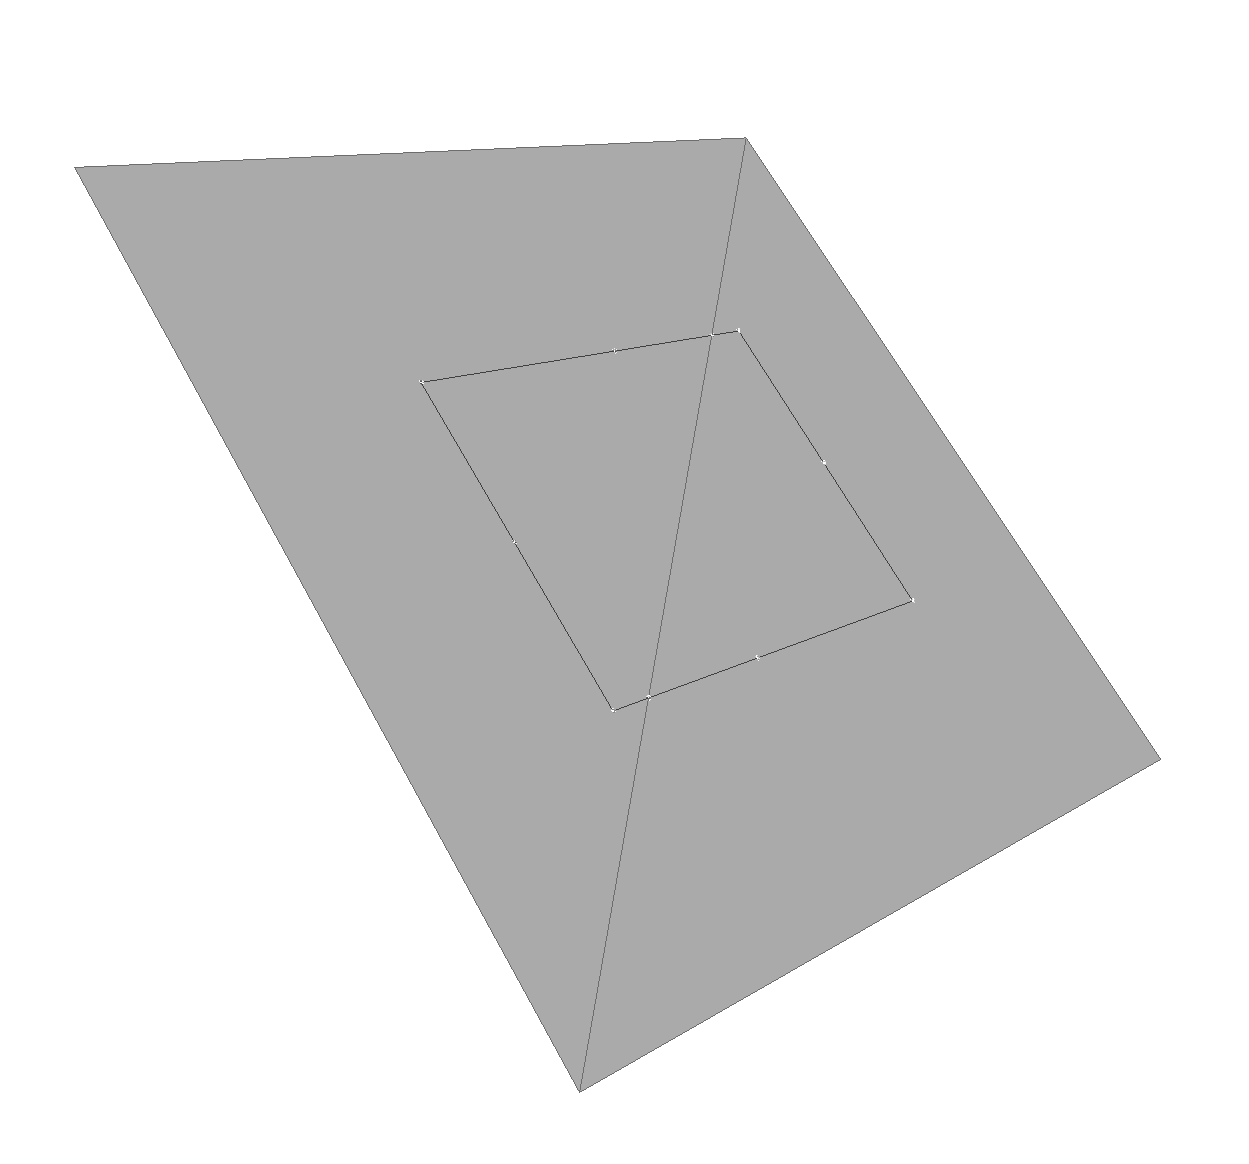
\includegraphics[width=\textwidth]{images/cube2_constraints}
		\caption{Intersections}
		\label{fig:cube2_constraints}
	\end{subfigure}
	\begin{subfigure}[t]{0.3\textwidth}
		\centering
		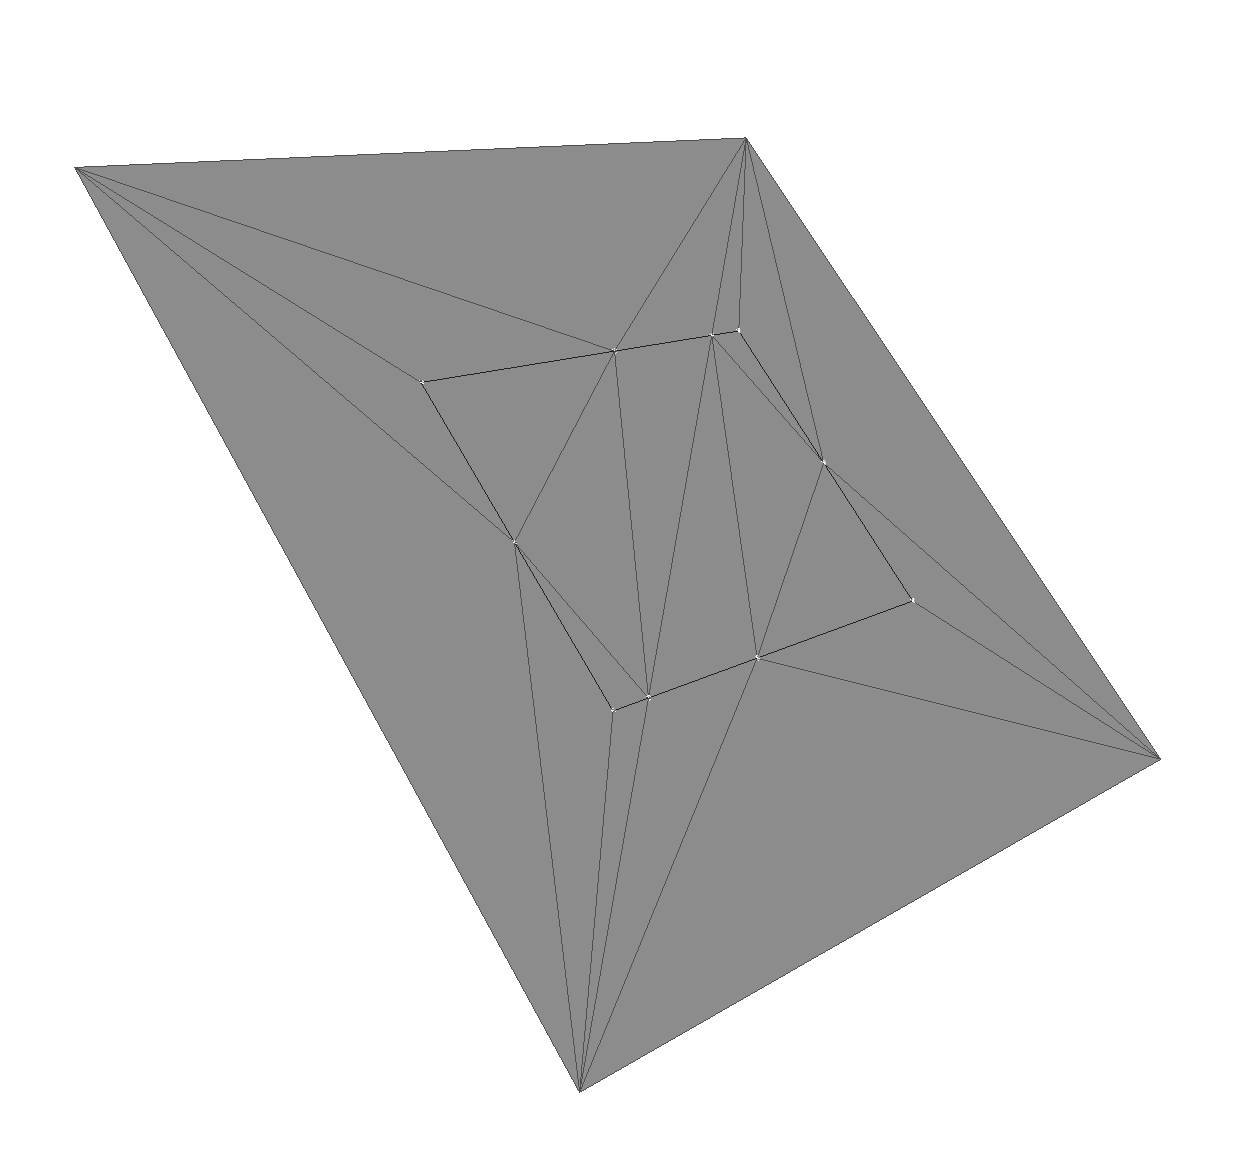
\includegraphics[width=\textwidth]{images/cube2_retriangulated}
		\caption{Retriangulation}
		\label{fig:cube2_retriangulated}
	\end{subfigure}
	\begin{subfigure}[t]{0.3\textwidth}
		\centering
		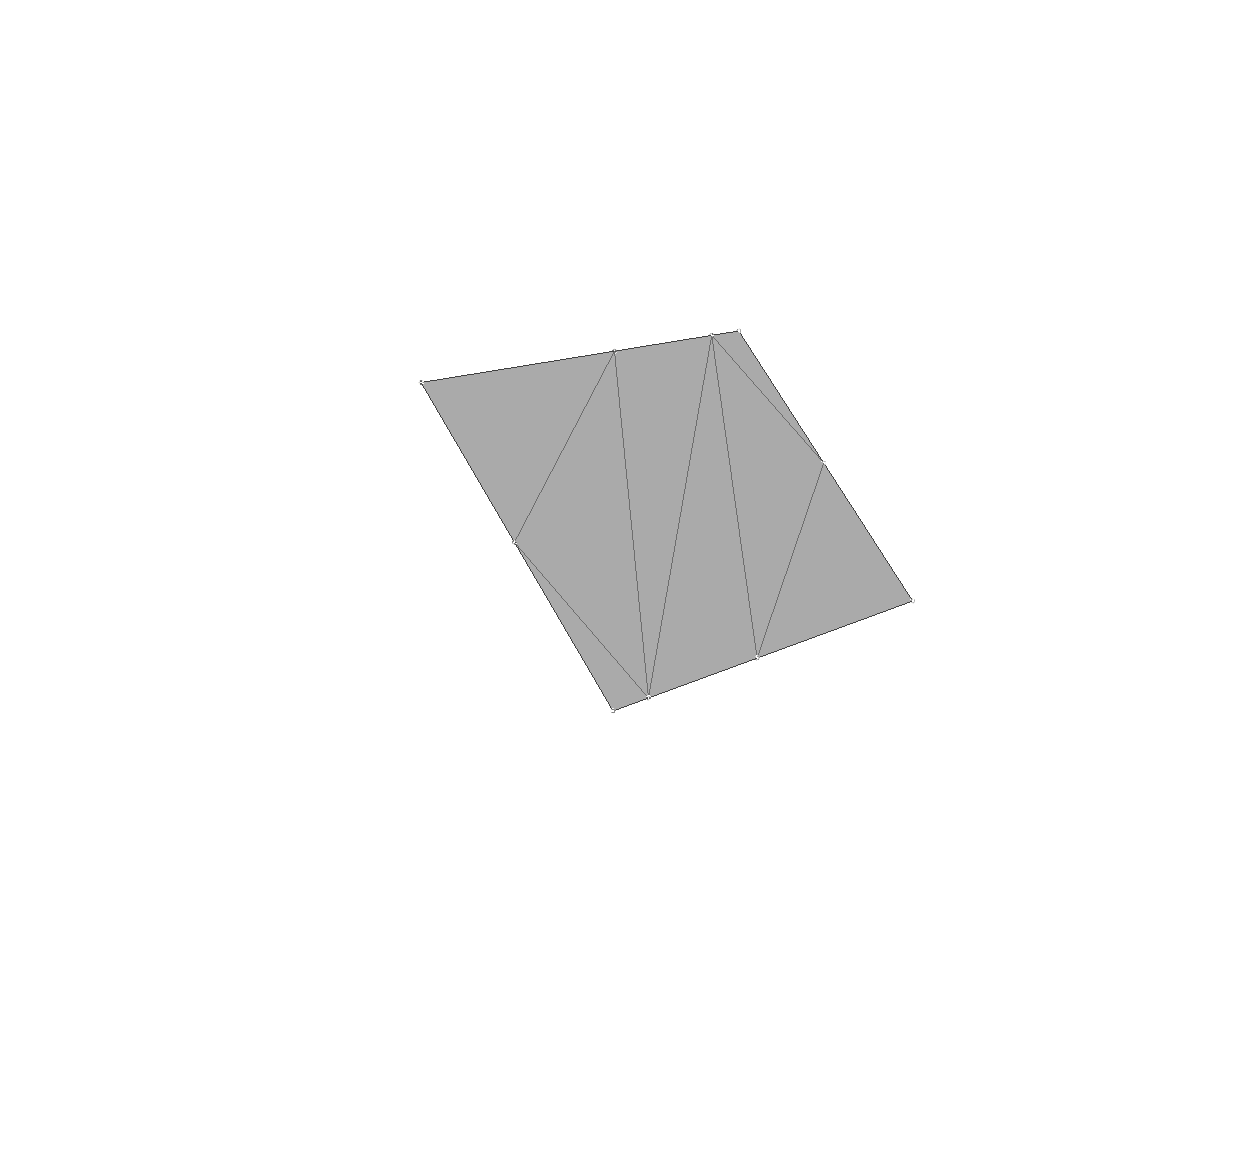
\includegraphics[width=\textwidth]{images/cube2_eliminated}
		\caption{Inside test}
		\label{fig:cube2_eliminated}
	\end{subfigure}
	\begin{subfigure}[t]{0.3\textwidth}
		\centering
		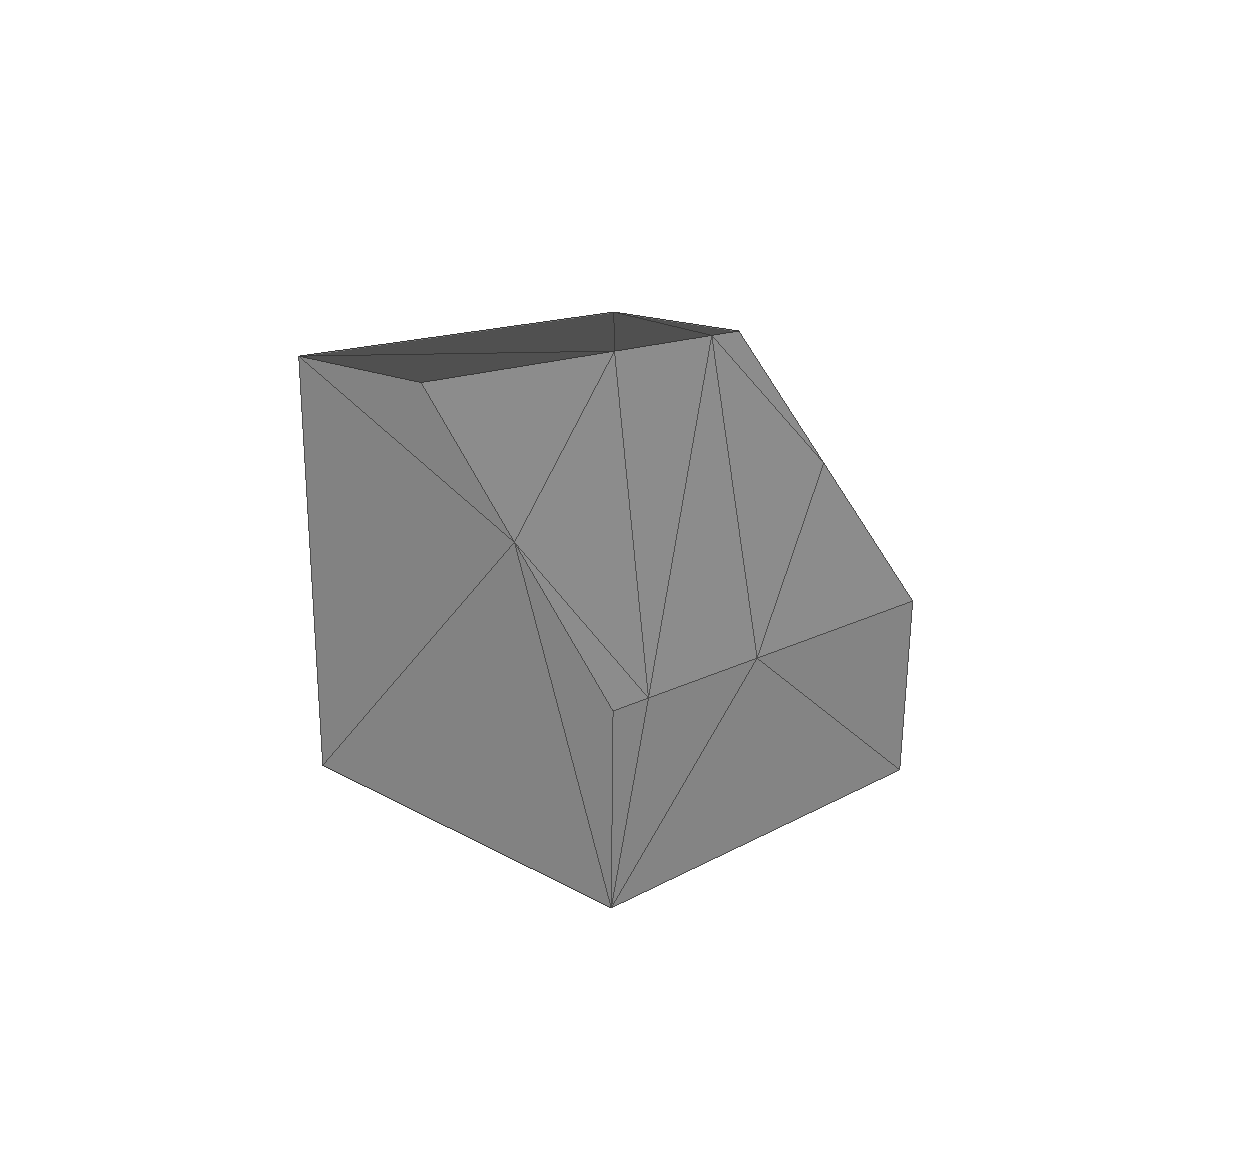
\includegraphics[width=\textwidth]{images/cube2_result}
		\caption{Result}
		\label{fig:cube2_result}
	\end{subfigure}
	\caption{
		Surface reconstruction from the VML's data model by the example of intersecting a cube and a cuboid.
		Figure \ref{fig:cube2_stock_sv} shows the cubic stock, in the lower left, and a tilted cuboid as swept volume, in the upper right.
		Figure \ref{fig:cube2_classified} shows the classification result when these two solids are mapped into the VML's regular grid.
		Most of the swept volume's triangles have been removed.
		When intersecting both structures, \ie swept volume and stock triangles, all intersection lines per triangle are recorded.
		Regarding the swept volume's triangles, these are shown in figure \ref{fig:cube2_constraints}.
		The triangles are then retriangulated with respect to those intersections as shown in figure \ref{fig:cube2_retriangulated}.
		Afterwards, each triangle is tested against the other structure, whether they are inside and can be removed.
		The result of testing the retriangulated swept volume's triangles against the stock is shown in figure \ref{fig:cube2_eliminated}.
		The retriangulation and inside test is analogously done for the stock structure.
		Finally, the reconstructed surface is the union of the remaining triangles, figure \ref{fig:cube2_result}.
	}
	\label{fig:cube2}
\end{figure}


\section{Implementation}
\label{sec:direct_intersection_implementation}

In general, intersecting each triangle of a structure against each other triangle of another structure is an expensive undertaking.
The cost of this operation is $\mathcal{O}(n^2)$, assuming both structures have $n$ triangles.
Intersecting the structures at the level of each cell greatly reduces the value of $n$.
Unfortunately, many triangles usually span the bounding box of a cell and are duplicated in each encompassed cell.
To avoid duplicates or overlapping triangles when combining results from neighboring cells, all triangles of a cell have to be clipped against the cell's bounding box.
This step can be done before or after intersecting the structures of a cell, but always before starting to eliminate triangles against the opposite structure.
There is also a second reason why this direct intersection approach must be run on a cell level which is discussed in section \ref{sec:triangle_inside_test}.

An abstracted algorithm of this reconstruction approach is shown in algorithm \ref{alg:direct_intersection}.
The following sections discuss details of this algorithms and follow the order of subroutines/functions which are not yet defined.
The only exception is the \textproc{SeparateStructures} routine, which only groups the incoming triangles by their structure id.
It returns a list of structures, where each structure is a set of triangles.

\begin{algorithm}
	\centering
	\begin{algorithmic}[1]
		\Function{DirectIntersection}{$\var{grid}$}
			\State $\var{result} \gets \varnothing$
			\ForAll{$\var{c} \in \var{grid.cells}$}
				\If{$\var{c.classification} = \var{surface}$}
					\State $\var{structures} \gets \Call{SeparateStructures}{\var{c.triangles}}$
					\If{$\left\vert{\var{structures}}\right\vert = 1$}
						\State $\var{result} \gets \var{result} \cup \Call{ClipStructure}{\var{structures.pop()}, \var{c.aabb}}$
					\ElsIf{$\left\vert{\var{structures}}\right\vert > 1$}
						\State $\var{acc} \gets \var{structures.pop()}$
						\While{$\left\vert{\var{structures}}\right\vert > 0$}
							\State $\var{s} \gets \var{structures.pop()}$
							\State $\var{acc} \gets \Call{UnionStructure}{\var{acc}, \var{s}, \var{c.aabb}}$
						\EndWhile
						\State $\var{result} \gets \var{result} \cup \var{acc}$
					\EndIf
				\EndIf
			\EndFor
			\State \Return $\var{result}$
		\EndFunction
		\\
		\Function{UnionStructure}{$\var{s_1}, \var{s_2}, \var{cellBox}$}
			\ForAll{$\var{s} \in \{\var{s_1}, \var{s_2\}}$}
				\State $s \gets \Call{ClipStructure}{\var{s}, \var{cellBox}}$
			\EndFor
			\State $\var{lines} \gets \var{map()}$ \Comment{maps each triangle to a set of lines}
			\ForAll{$(\var{t_1}, \var{t_2}) \in \var{s_1} \times \var{s_2}$}
				\State $\var{l} \gets \Call{IntersectTriangles}{\var{t_1}, \var{t_2}}$
				\If{$\var{l}$} \Comment{no intersection line may be found}
					\State $\var{lines}(\var{t_1}) \gets \var{lines}(\var{t_1}) \cup \{\var{l}\}$
					\State $\var{lines}(\var{t_2}) \gets \var{lines}(\var{t_2}) \cup \{\var{l}\}$
				\EndIf
			\EndFor
			\ForAll{$\var{s} \in \{\var{s_1}, \var{s_2}\}$}
				\State $\var{s'} \gets \varnothing$
				\ForAll{$\var{t} \in \var{s}$}
					\State $\var{s'} \gets \var{s'} \cup \Call{SplitTriangle}{\var{t}, \var{lines}(\var{t})}$
				\EndFor
				\State $\var{s} \gets \var{s'}$
			\EndFor
			\State $\var{result} \gets \varnothing$
			\ForAll{$(\var{s}, \var{s'}) \in \{(\var{s_1}, \var{s_2}), (\var{s_2}, \var{s_1})\}$}
				\ForAll{$\var{t} \in \var{s}$}
					\If{$\neg \Call{IsTriangleInsideStructure}{\var{t}, \var{s'}}$}
						\State $\var{result} \gets \var{result} \cup \{\var{t}\}$
					\EndIf
				\EndFor
			\EndFor
			\State \Return $\var{result}$
		\EndFunction
	\end{algorithmic}
	\caption{
		Abstract workflow of the surface extraction using direct intersection of the VML's stored structures.
	}
	\label{alg:direct_intersection}
\end{algorithm}


\subsection{Clipping}
\label{sec:clipping}

Clipping triangles against the bounding box of a cell is necessary to avoid duplicated or invalid surfaces.
In cases where triangles span multiple cells, the VML duplicates each triangle into each cell it encompasses.
During intersection, only a triangle's intersections with structures of the current cell are recorded, although the triangle might be intersected by additional geometry in neighboring cells.
Therefore, after splitting, parts of the triangle which are outside the current cell are never split, might pass the inside test as a whole and remain as additional triangles outside the actual surface or remain colinear with surface triangles from neighboring cells.
To circumvent these issues, all triangles of a cell have to be clipped either before or after intersecting the two structures in \textproc{UnionStructure}.

Algorithms for clipping triangles against a bounding box are found in literature.
A well-known examples is the Sutherland-Hodgeman algorithm for polygon clipping \cite{polygon_clipping}.
Although further algorithms exist, \eg Weiler-Artherton, Vatti or Greiner-Hormann, which are either faster, more robust or have fewer restrictions on their input, the Sutherland-Hodgeman algorithm is characteristically simple.
In particular, it clips any polygon against any convex clip polygon by iteratively clipping it against infinitely extended lines along each edge of the clip polygon.
Despite being initially designed for 2 dimensions, the algorithm easily extends to higher dimensions.

For clipping triangles against the bounding box of a cell, a 3-dimensional version of the Sutherland-Hodgeman algorithm is needed.
Algorithm \ref{alg:clip} shows a pseudocode implementation of the \textproc{ClipStructure} routine which is based on the Sutherland-Hodgeman algorithm to clip all structure triangles against the bounding box of a cell.
%
When clipping a structure against a bounding box, each individual triangle of the structure is clipped separately.
The result of clipping a single triangle may be the same triangle, a set of new triangles or even no triangle at all.
The resulting triangles after clipping, if any, are collected to form the new, clipped structure.

The Sutherland-Hodgeman algorithm clips against a convex polygon, or its equivalent in higher dimensions, \ie a polytope, by iteratively clipping against each side.
In case of a bounding box, the input polygon has to be clipped against each of the six sides of the cell.
These sides are extended and described as planes by specifying a normal vector and the plane's distance to the origin.
The six planes built from a cell's bounding box are given in the \textproc{ClipPolygonAABB} function of algorithm \ref{alg:clip}.
The input polygon itself is represented as an ordered list of vertices, where each pair of adjacent vertices form an edge of the polygon, including the last and the first vertex as a pair.
The order of the vertices remains the sames during the clipping process, but vertices may be removed or additional ones added.
The final vertex list, after clipping against all planes, needs to be triangulated again.
As the clipping volume, \ie the cell's bounding box, is convex, the resulting clipped polygon is also convex.
Therefore, the list of vertices can be simply triangulated into a fan by selecting one vertex and emitting a triangle for every adjacent pair of vertices excluding the selected vertex, where each triangle is built from the pair and the selected vertex.
Note that in some edge cases, duplicate vertices may be generated.
Thus, duplicates should be removed from the result vertex list before passing it to the triangulation subroutine.

The core routine of the clipping procedure is clipping the list of vertices against a single plane.
Initially, an empty list of result vertices is created.
For each of the polygon's vertices, the signed distance to the clipping plane is calculated.
The distance of each vertex is compared with the distance of its preceding vertex.
If the signs of the distances are different, the edge represented by the current vertex and its predecessor intersects the clipping plane.
In this case, the intersection point with the clipping plane is calculated, \cf algorithm \ref{alg:clip} for details, and the point is added to the result list.
If the distance of the current vertex is positive, the vertex itself is inside the clipping volume and is also added to the result list.
After all vertices have been processed, the result list is return, representing the clipped polygon again as an ordered list of its vertices.

\begin{algorithm}
	\centering
	\begin{algorithmic}[1]
		\Function{ClipStructure}{$\var{s}, \var{aabb}$}
			\State $\var{s'} \gets \varnothing$
			\ForAll{$\var{t} \in \var{s}$}
				\State $\var{s'} \gets \var{s'} \cup \Call{ClipPolygonAABB}{\var{t.vertices}, \var{aabb}}$
			\EndFor
			\State \Return $\var{s'}$
		\EndFunction
		\\
		\Function{ClipPolygonAABB}{$\var{vertices}, \var{aabb}$}
			\State $\var{vertices} \gets \Call{ClipPolygonPlane}{\var{vertices}, \var{Vertex}( 1, 0, 0), \var{aabb.lower.x}}$
			\State $\var{vertices} \gets \Call{ClipPolygonPlane}{\var{vertices}, \var{Vertex}(-1, 0, 0), \var{aabb.upper.x}}$
			\State $\var{vertices} \gets \Call{ClipPolygonPlane}{\var{vertices}, \var{Vertex}( 0, 1, 0), \var{aabb.lower.y}}$
			\State $\var{vertices} \gets \Call{ClipPolygonPlane}{\var{vertices}, \var{Vertex}( 0,-1, 0), \var{aabb.upper.y}}$
			\State $\var{vertices} \gets \Call{ClipPolygonPlane}{\var{vertices}, \var{Vertex}( 0, 0, 1), \var{aabb.lower.z}}$
			\State $\var{vertices} \gets \Call{ClipPolygonPlane}{\var{vertices}, \var{Vertex}( 0, 0,-1), \var{aabb.upper.z}}$
			
			\State \Return $\Call{Trianglulate}{\Call{Unique}{\var{vertices}}}$
		\EndFunction
		\\
		\Function{ClipPolygonPlane}{$\var{vertices}, \var{n}, \var{d}$}
			\State $\var{result} \gets \var{array}()$
			\State $\var{prev} \gets |\var{vertices}| - 1$
			\State $\var{prevDist} \gets \var{vertices_{prev}} * \var{n} - \var{d};$
			\For{$\var{i} \gets 0, \dots, |\var{vertices}| - 1$}
				\State $\var{dist} \gets \var{vertices_i} * \var{n} - \var{d}$;
				\If{$(\var{dist} < 0 \wedge \var{prevDist} \geq 0) \vee (\var{dist} \geq 0 \wedge \var{prevDist} < 0)$}
					\State $\var{edge} \gets (\var{vertices_i} - \var{vertices_{prev}})$
					\State $\var{edge} \gets \var{edge} * \frac{\var{dist}}{\var{n} * \var{edge}}$
					\State $\var{v} \gets \var{vertices_i} - \var{edge}$
					\State $\var{result.add}(\var{v})$
				\EndIf
				\If{$\var{dist} \geq 0$}
					\State $\var{result.add}(\var{vertices_i});$
				\EndIf
				\State $\var{prev} \gets i$;
				\State $\var{prevDist} \gets \var{dist}$;
			\EndFor
			\State \Return $\var{result}$
		\EndFunction
		\\
		\Function{Triangulate}{$\var{vertices}$}
			\State $\var{result} \gets \varnothing$
			\If{$|vertices| \geq 3$}
				\State $\var{c} \gets \var{loop_0}$
				\For{$\var{i} \gets 2, \dots, |\var{vertices}| - 1$}
					\State $\var{result} \gets \var{result} \cup \{\var{Triangle}(\var{c}, \var{vertices_{i - 1}}, \var{vertices_i})\}$
				\EndFor
			\EndIf
			\State \Return $\var{result}$
		\EndFunction
	\end{algorithmic}
	\caption{
		A Sutherland-Hodgeman algorithm variant for clipping polygons against a bounding box in 3 dimensions.
	}
	\label{alg:clip}
\end{algorithm}



\subsection{Triangle intersection}
\label{sec:triangle_intersection}

Every time the union surface of two structures is calculated, each triangle of one structure has to be intersected with each triangle of the other structure.
Triangle-triangle intersection is a common problem in collision detection and has been solved numerous times.
The intersection test of Möller \cite{tri_tri_intersection_moller}, despite being older and marginally slower than more recent developments \cite{tri_tri_intersection_2}, is also available as public domain C code on the authors website \cite{tri_tri_intersection_moller_code}.
As only a few adaptations were necessary, Möller's code was taken and thoroughly refactored to fit a modern C++ style without changing its behavior.
Since the code is quite long and freely available on Möller's website, an implementation/algorithm is not included here.
The \textproc{IntersectTriangle} routine referenced in algorithm \ref{alg:direct_intersection} is thus merely a small adapter calling into Möller's code and is given in algorithm \ref{alg:triangle_intersection}.

\begin{algorithm}
	\centering
	\begin{algorithmic}[1]
		\Function{IntersectTriangles}{$\var{t_1}, \var{t_2}$}
			\State $\var{isCoplanar}, \var{p_1}, \var{p_2}$ \Comment{Uninitialized variables}
			\State $\var{hasIntersected} =$ \Call{tri\_tri\_intersect\_with\_isectline}{$\hfill\break
				% the phantoms at the line starts make sure all hspaces start at the same position
				\protect\vphantom{p}\hspace*{\dimexpr\algorithmicindent*2}\var{t_1.vertices_0}, \var{t_1.vertices_1}, \var{t_1.vertices_2},\hfill\break
				\protect\vphantom{p}\hspace*{\dimexpr\algorithmicindent*2}\var{t_2.vertices_0}, \var{t_2.vertices_1}, \var{t_2.vertices_2},\hfill\break
				\protect\vphantom{p}\hspace*{\dimexpr\algorithmicindent*2}\var{coplanar}, \var{p_1}, \var{p_2}$}
			\If{$hasIntersected \wedge \neg isCoplanar$}
				\State \Return $(\var{p_1}, \var{p_2})$ \Comment{Otherwise return nothing}
			\EndIf
		\EndFunction
	\end{algorithmic}
	\caption{
		Adapter to the Möller's triangle intersection routine provided as public domain C code on his website \cite{tri_tri_intersection_moller_code}.
		This algorithm calls the C function \textproc{tri\_tri\_intersect\_with\_isectline} with all triangle vertices as inputs and $\var{coplanar}$, $\var{p_1}$ and $\var{p_2}$ as output parameters.
	}
	\label{alg:triangle_intersection}
\end{algorithm}

The triangle intersection test itself starts with an early exit test by computing the plane equation parameters, \ie normal and distance, for both triangles.
Then, the signed plane distance of each vertex of one triangle to the plane of the other triangle is calculated.
If the signs of these three values is the same for one triangle, it completely lies on one side of the plane and therefore does not intersect the other triangle.
This test is run for both triangles.
Afterwards, the intersection line between the two planes is calculated by crossing the planes' normal vectors.
Figure \ref{fig:tri_intersect} shows the intersection line of the two triangle planes in green and is used to discuss the remaining part of the algorithm.
Now, the intervals of the line which lie inside the triangle have to be calculated.
For each pair of vertices of a triangle, \ie each triangle's edges, the two signed distances of the vertices to the plane of the other triangle are compared.
If they have a different sign, this edge intersects the other triangle's plane and therefore crosses the intersection line of both planes.
The intersection point splits the edge with the same ratio as the signed distances of both vertices.
For each triangle, two intersecting edges are found, thus yielding an interval for each triangle, \cf blue segments of the line in figure \ref{fig:tri_intersect}.
If these two intervals overlap, the triangles intersect and their intersection line is the overlapping segment of the planes' intersection line, \cf red segment in figure \ref{fig:tri_intersect}.
Otherwise, there is no intersection.

\begin{figure}
	\centering
	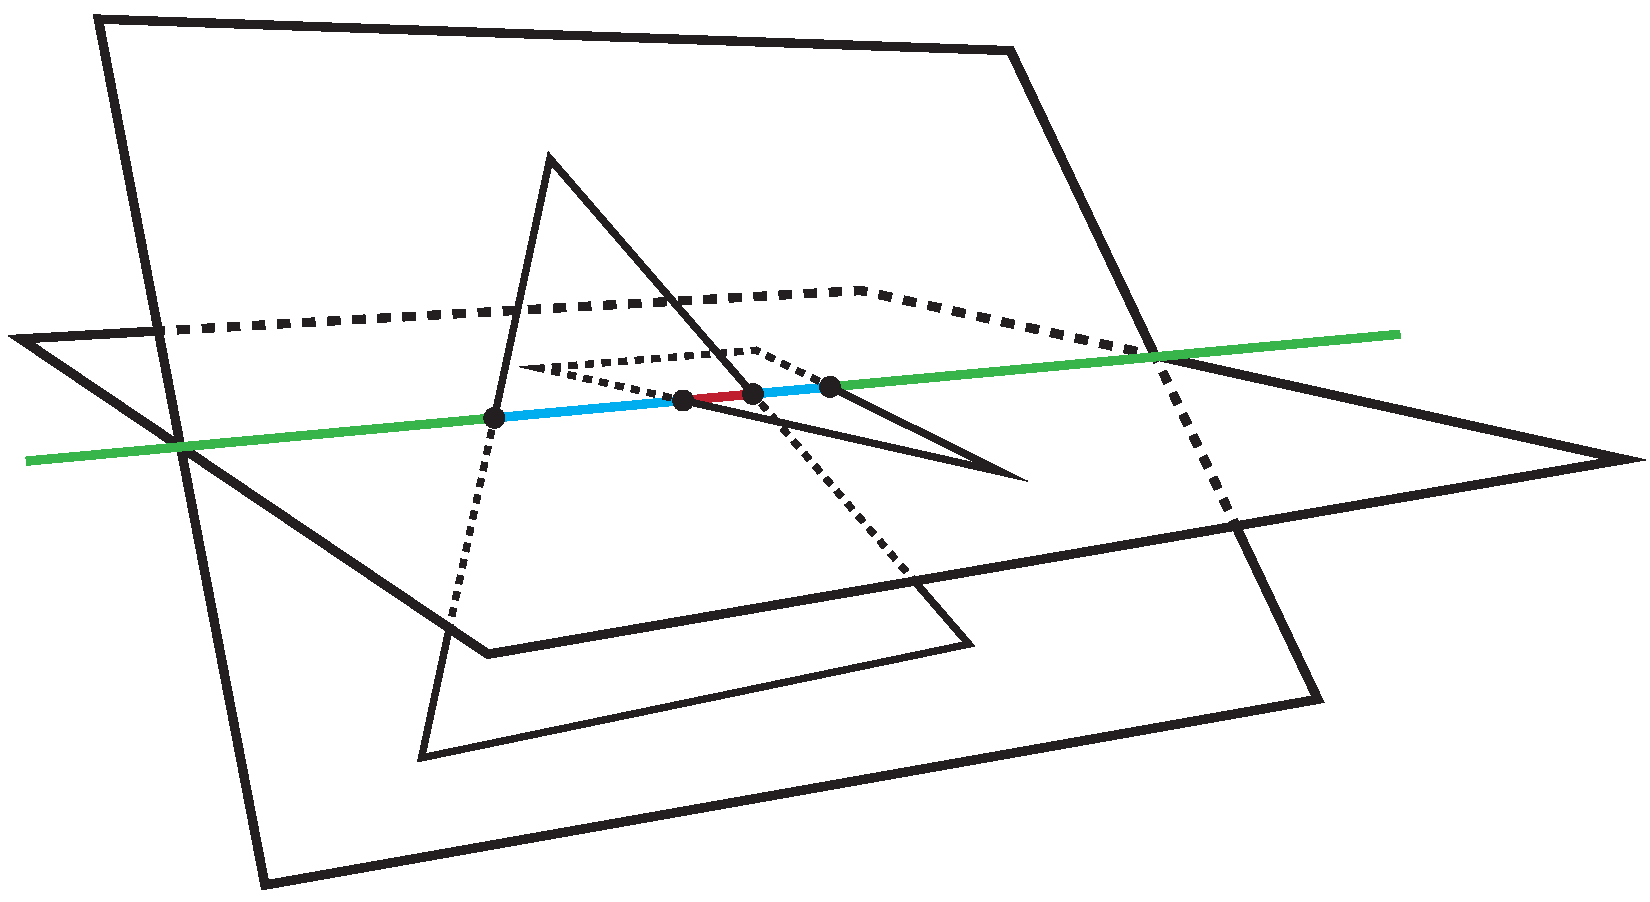
\includegraphics[width=0.8\textwidth]{tri_intersect}
	\caption{
		Intersection line calculation in Möller's triangle intersection test.
		The image shows intervals on the intersection line between two triangle's planes.
		The green line is the intersection line of both planes.
		Blue parts of the intersection line are intervals of one triangle.
		The red part is the overlap of both triangle's line intervals, \ie the triangle's intersection.
		Image modeled after \cite[p757]{tri_tri_intersection_moller_image}.
	}
	\label{fig:tri_intersect}
\end{figure}

Extending beyond this concept, a further optimization is to do not use the planes' intersection line to project the triangle's intervals onto, but to use the coordinate system's axis where the intersection line's direction has the largest magnitude.
This greatly simplifies several calculations except the actual points of the intersection segment.
Furthermore, Möller's code additionally handles the case when both triangles are coplanar, \ie the signed distances of the vertices of one triangle to the other triangle's plane are almost zero.



\subsection{Triangle splitting}
\label{sec:triangle_splitting}

After two structures have been intersected and all intersection lines per triangle have been recorded, the triangles can be split.
The result of splitting a triangle must be a new set of triangles in order to create a new structure from these which can be put into the \textproc{UnionStructure} routine again.
Hence, an algorithm for triangulating a triangle with respect to a set of lines is needed.
In the context of triangulations, this set of lines is usually called constraints or constrained edges and the according algorithm a constrained triangulation (CT).
Initially, a manually written CT was used.
Even though it was capable of triangulating simple cases, it suffered severely from numerical instability and poor output quality.
A stricter triangulation of higher quality is the constrained Delaunay triangulation (CDT), which is also suggested by the paper giving the initial idea to this approach \cite{mesh_intersection}.
However, as CDT algorithms are quite hard to implement regarding speed and robustness, using an established and tested library is highly recommended.
A list of C/C++ libraries offering constrained Delaunay triangulations is given in table \ref{tbl:delaunay_libs}.
Several of these libraries have been tested for their suitability to retriangulate a triangle with a set of constraints.
Usually, these triangulation algorithms operate on 2-dimensional point clouds with optional constrained edges between points of this cloud.
As output they generate a Delaunay mesh, with the convex hull of the point cloud as boundary.

\renewcommand{\arraystretch}{1.5} % row spacing
\begin{table}[h]
	\centering
	\begin{tabular}{p{3cm} l l p{2.1cm} p{3.9cm}}
		Library                                          &                           & Language & License                                  & Notes                                                             \\
		\hline
		poly2tri                                         & \cite{poly2tri}           & C++      & BSD                                      & Constrains via polylines must not touch each other                \\
		Triangle                                         & \cite{triangle_lib}       & C        & Custom, free for non-commercial use      & Difficult interface and memory management                         \\
		Geometric Tools Engine (GTE)                     & \cite{gte}                & C++      & Boost License                            & modern C++11, SIMD and GPGPU support, high standard documentation \\
		Computational Geometry Algorithms Library (CGAL) & \cite{cgal_triangulation} & C++      & LGPL, GPL or commercial                  & Huge functionality, de-facto standard in academics                \\
		Fade2D                                           & \cite{fade2d}             & C++      & Commercial, free for scientific research & Closed source                                                     \\
		Triangulation Template Library (TTL)             & \cite{ttl}                & C++      & GPL                                      & Supports usage of own data structures via C++ templates           \\
		GNU Triangulated Surface Library (GTS)           & \cite{gts}                & C        & LGPL                                     & object-oriented design using GLib                                 \\
	\end{tabular}
	\caption{
		Table containing several libraries offering a constrained Delaunay triangulation.
	}
	\label{tbl:delaunay_libs}
\end{table}
\renewcommand{\arraystretch}{1.0}

The poly2tri library requires constraints to be specified as polylines which may not touch each other.
This is a problem as constraints may touch the boundary of the original triangle.
%
The Triangle library has been used for exactly this purpose in another paper \cite{mesh_intersection}.
Nevertheless, it has a very difficult C interface which tries to mimic a command line with text arguments even on API level.
Furthermore, passing in and returning geometric data structures requires extensive care regarding memory management.
The library did work for most of the cases but crashed several times, \eg on every 1000\textsuperscript{th} triangle.  
%
The Geometric Tools Engine (GTE) is a rather modern library with an excellent C++ interface.
The algorithms' precision may be configured via templates.
The library runs outstandingly stable with only a few troubles in cases where the input was numerically problematic, \eg contained points with differences only at the last few digits representable with double precision.
However, these issues can be fixed with appropriate preprocessing of the input, \cf section \ref{sec:numeric_improvements}.
Furthermore, the GTE library is licensed under the Boost License and therefore perfectly usable in commercial products like the VML.
%
The remaining libraries have not been further tested, mainly for the reason that the VML is a commercial product and the use of these libraries would require to drop the code again later.

The integration of the GTE's CDT is done inside \textproc{SplitTriangle} which is given in algorithm \ref{alg:triangle_splitting}.
%
\begin{algorithm}
	\centering
	\begin{algorithmic}[1]
		\Function{SplitTriangle}{$\var{t}, \var{lines}$}
			\State $\var{points} \gets \{\var{t.a}, \var{t.b}, \var{t.c}\}$ \Comment{Ordered set}
			\ForAll{$\var{(p_1, p_2)} \in \var{lines}$}
				\State $\var{points} \gets \var{points} \cup \{\var{p_1}, \var{p_2}\}$
			\EndFor
			\State $\var{axis_0} \gets \Call{LargestAxis}{t.normal}$
			\State $\var{axis_1} \gets (axis_0 + 1) \bmod 3$ 
			\State $\var{axis_2} \gets (axis_0 + 2) \bmod 3$
			\State $\var{points2} \gets \varnothing$ \Comment{Project 3D to 2D points, order must remain}
			\ForAll{$\var{p} \in points$}
				\State $\var{points2} \gets \var{points2} \cup \{\var{Vector2}(\var{p_{axis1}}, \var{p_{axis2}})\}$
			\EndFor
			\State $\var{cdt} \gets \var{ConstrainedDelaunay2()}$
			\ForAll{$(\var{p_1}, \var{p_2}) \in \var{lines}$} \Comment{Add constraints}
				\State $\var{cdt.Insert}((\var{points.indexof}(\var{p_1}), \var{points.indexof}(\var{p_2})), \dots)$
			\EndFor
			\State $\var{cdt}(|\var{points2}|, \var{points2}, \epsilon)$ \Comment{Compute CDT}
			\State $\var{indices} \gets \var{cdt.GetIndices()}$
			\State $\var{triangles} \gets \varnothing$
			\For{$\var{i} \gets 0,\dots,\frac{|\var{indices}|}{3} - 1$}
				\State $\var{f} \gets \var{triangle()}$
				\For{$\var{j} \gets 0,1,2$}
					\State $\var{index} \gets \var{indices_{i * 3 + j}}$
					\State $\var{f_j} = \var{points_{index}}$
				\EndFor
				%\If{$\var{f.normal} * \var{t.normal} < 0$}
				%	\State $\var{swap}(\var{f.a}, \var{f.b})$ \Comment{Swap two vertices to reverse winding}
				%\EndIf
				\State $\var{triangles} \gets \var{triangles} \cup \{\var{f}\}$
			\EndFor
			\State \Return $\var{triangles}$
		\EndFunction
		\\
		\Function{LargestAxis}{$\var{v}$}
			\If{$\var{v.x} > \var{v.y}$}
				\If{$\var{v.x} > \var{v.z}$}
					\State \Return $0$
				\Else
					\State \Return $2$
				\EndIf
			\Else 
				\If{$\var{v.y} > \var{v.z}$}
					\State \Return $1$
				\Else
					\State \Return $2$
				\EndIf
			\EndIf
		\EndFunction
	\end{algorithmic}
	\caption{
		Adapter to the CDT routine provided by the GTE library.
		Uses the $\var{ConstrainedDelaunay2}$ class template to generate a CDT for a given triangle and a set of constrained edges.
		The resulting triangulation is returned.
	}
	\label{alg:triangle_splitting}
\end{algorithm}
%
A few preparations are necessary before the CDT subroutine can be called.
All points used by constrained edges must be part of the input point cloud and are therefore added to the point cloud formed by the input triangle's vertices.

Furthermore, as the CDT only runs in 2 dimensions, all vertices are projected onto the plane spanned by the two coordinate system axes with the smaller magnitude in the triangle's normal vector.
This operation is simple as it only requires the selection of two components of each point and no calculation.
As all constraints as well as the resulting triangulation are specified using indexes into the point cloud, the list containing the 2-dimensional, projected vertices must have the same order as the original point list.
Before starting the triangulation, the constrained edges have to be specified.
Each constraint is inserted by supplying a pair of indexes into the point cloud.
Afterwards, the CDT can be calculated.
The resulting triangulation is specified using a list of indexes.
The length of this list is a multiple of 3 and each consecutive 3 indexes form a triangle of the result.
When these indexes are resolved by indexing into the original point cloud, the vertices for the final triangles are obtained.
These triangles are finally returned.


\subsection{Triangle inside structure test}
\label{sec:triangle_inside_test}

After all triangles of two intersecting structures have been split on their intersection lines, all triangles which do not contribute to the union surface, \ie are inside the other structure, have to be removed.
Due to the regular grid's classification, \cf section \ref{sec:classification}, triangles might have been removed and, consequently, structures put together from multiple cells of the regular grid may no longer be closed meshes.
As it turns out, the test whether a triangle is inside another structure may fail if the tested structure is not a closed mesh, a common case.
An example of such an issue is shown in figure \ref{fig:inside_test_error}.
%
\begin{figure}[!]
	\centering
	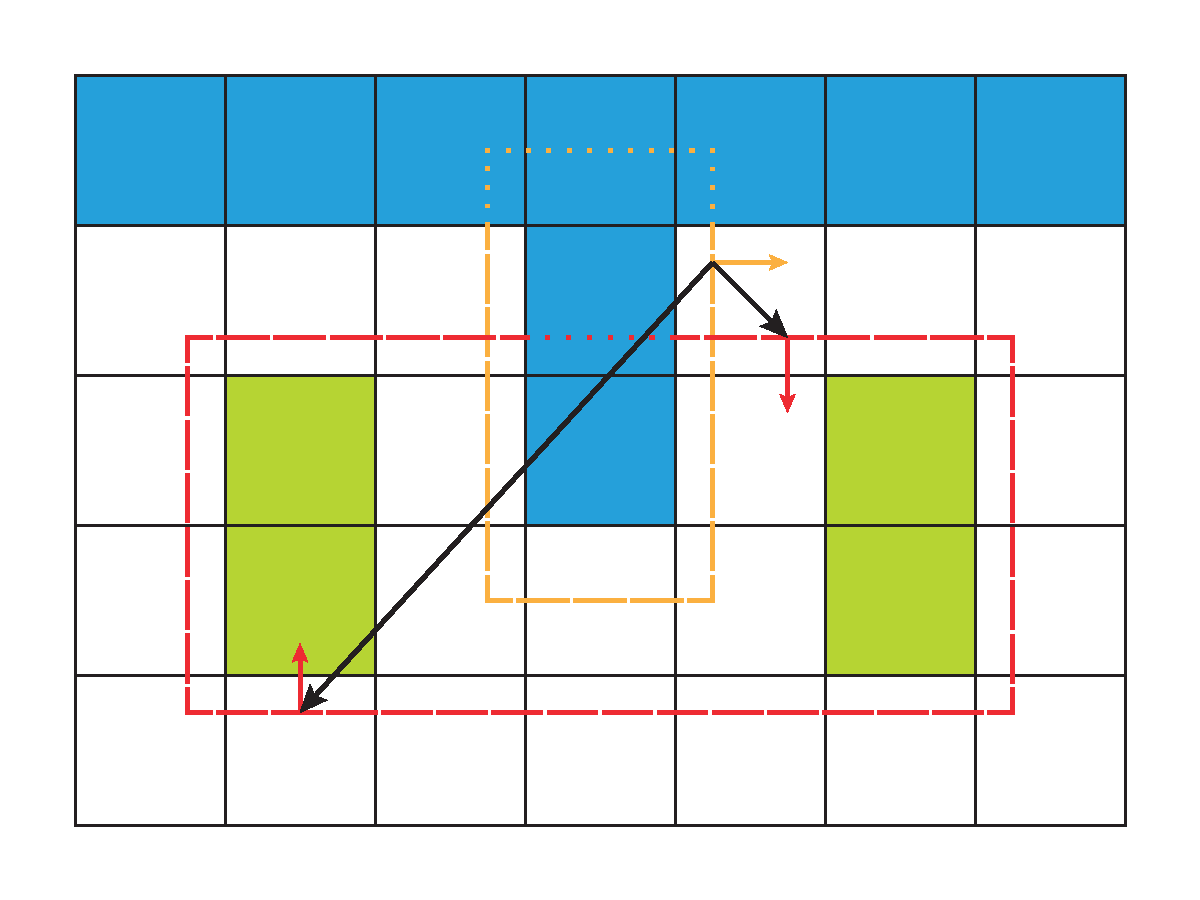
\includegraphics[width=0.8\textwidth]{inside_test_error}
	\caption{
		Testing if a triangle of one structure is inside another structure using a ray.
		Due to triangle elimination, the ray can miss removed structures, \eg when traversing outside cells, causing the inside test to fail, \cf left ray.
		As structures are guaranteed to be closed within a cell, this test is only valid within a cell, \cf right ray.
	}
	\label{fig:inside_test_error}
\end{figure}
%
A triangle is tested against a structure by using a ray.
This ray is shot from an arbitrary point on the triangle, which does not lie on an edge, \eg the triangle's centroid, to an arbitrary point on a triangle of the other structure.
If the ray does not intersect the other structure on its way, a comparison of the ray's direction with the normal of the targeted triangle determines whether the ray's origin, \ie the centroid of the tested triangle, is inside the other structure or not.
However, as classification might eliminate triangles, the ray could potentially intersect triangles of the structure which have been removed, \cf left ray in figure \ref{fig:inside_test_error}.
The regular grid only guarantees closed meshes within a cell.
To circumvent this issue, the inside test for a triangle must be conducted within a cell.

An algorithm for this \textproc{IsTriangleInsideStructure} test is given in algorithm \ref{alg:triangle_inside_test}. 
%
\begin{algorithm}
	\centering
	\begin{algorithmic}[1]
		\Function{IsTriangleInsideStructure}{$\var{t}, \var{s}$}
			\State $\var{origin} \gets \frac{\var{t.a} + \var{t.b} + \var{t.c}}{3}$ \Comment{Origin is triangle center}
			\State $\var{target} \gets \frac{\var{s_0.a} + \var{s_0.b} + \var{s_0.c}}{3}$ \Comment{Target ray at center of $\var{s_0}$}
			\State $\var{ray} \gets \var{target} - \var{origin}$
			\State $\var{d_{nearest}} \gets \var{ray.length}()$
			\State $\var{n_{nearest}} \gets \var{s_0.normal}$
			\State $\var{raydir} \gets \var{ray.normalized()}$
			\ForAll{$\var{f} \in \var{s} \setminus \{\var{s_0}\}$} \Comment{Retarget ray at closer triangle if intersected}
				\State $\var{d}, \var{u}, \var{v}$
				\If{$\Call{IntersectRayTriangle}{\var{origin}, \var{raydir}, \var{f}, \var{d}, \var{u}, \var{v}}$}
					\If{$\var{d} > 0 \wedge \var{d} < \var{d_{nearest}}$}
						\State $\var{d_{nearest}} \gets \var{d}$
						\State $\var{n_{nearest}} \gets \var{f.normal}$
					\EndIf
				\EndIf
			\EndFor
			\State \Return $\var{n_{nearest}} * \var{rayDir} \geq 0$
		\EndFunction
		\\
		\Function{IntersectRayTriangle}{$origin, direction, t, d, u, v$}
			\State $\var{vertex_0} \gets \var{t.a}$
			\State $\var{edge_1} \gets \var{t.b} - \var{t.a}$
			\State $\var{edge_2} \gets \var{t.c} - \var{t.a}$
			\State $\var{tVec} \gets \var{origin} - \var{vertex_0}$
			\State $\var{pVec} \gets \var{direction} \times \var{edge_2}$
			\State $\var{det} \gets \var{edge_1} \cdot \var{pVec}$
			\State $\var{u} \gets \var{tVec} \cdot \var{pVec}$
			\State $\var{qVec} \gets \var{tVec} \times \var{edge_1}$
			\State $\var{v} \gets \var{qVec} *\cdot \var{direction}$
			\State $\var{invDet} \gets \frac{1}{\var{det}}$
			\State $\var{distance} \gets \var{edge_2} \cdot \var{qVec} \cdot \var{invDet}$
			\State $\var{u} \gets \var{u} \cdot \var{invDet}$
			\State $\var{v} \gets \var{v} \cdot \var{invDet}$
			\State \Return $(\var{u} \geq 0) \wedge (\var{v} \geq 0) \wedge (\var{u} + \var{v} \leq 1)$
		\EndFunction
	\end{algorithmic}
	\caption{
		Algorithm for testing whether a triangle is inside another structure.
		The \textproc{IntersectRayTriangle} function is a branch-free version of the famous Möller-Trumbore ray-triangle intersection test \cite{ray_triangle_intersection_moller}.
	}
	\label{alg:triangle_inside_test}
\end{algorithm}
%
The function starts by calculating the origin and target point for the test ray.
The ray originates the center of the tested triangle and initially targets the center of the first triangle of the other structure.
Distance and normal of the targeted triangle are stored.
Then, all other triangles of the structure are tested for intersection with the created ray.
If an intersection happens and the distance to the newly intersected triangle is shorter than the distance to the currently targeted triangle, the distance and normal are updated to the new triangle, \ie the ray now targets the new triangle.
This procedure ensures that after all triangles have been tested for intersection, the maintained distance and normal store the values of the closest intersection of the ray.
The normal of the closest intersected triangle of the other structure is then finally compared to the ray's direction.
If they point into the same half space, the ray's origin and therefore the tested triangle is inside the tested structure.

For ray-triangle intersection the famous Möller-Trumbore intersection test is used \cite{ray_triangle_intersection_moller}.
An implementation of their algorithm in C is already given in the corresponding paper.
The original version has a few early exit tests on $u$ and $v$, which might save some work in case the ray misses the triangle.
However, branching is becoming increasingly expensive on modern hardware architectures, especially in vectorized code paths or GPU code.
A branch-free version of Möller-Trumbore's code, which is currently used and performs slightly better, is shown in algorithm \ref{alg:triangle_inside_test}.

The idea of the algorithm is shown in figure \ref{fig:ray_triangle_intersect}.
%
\begin{figure}
	\centering
	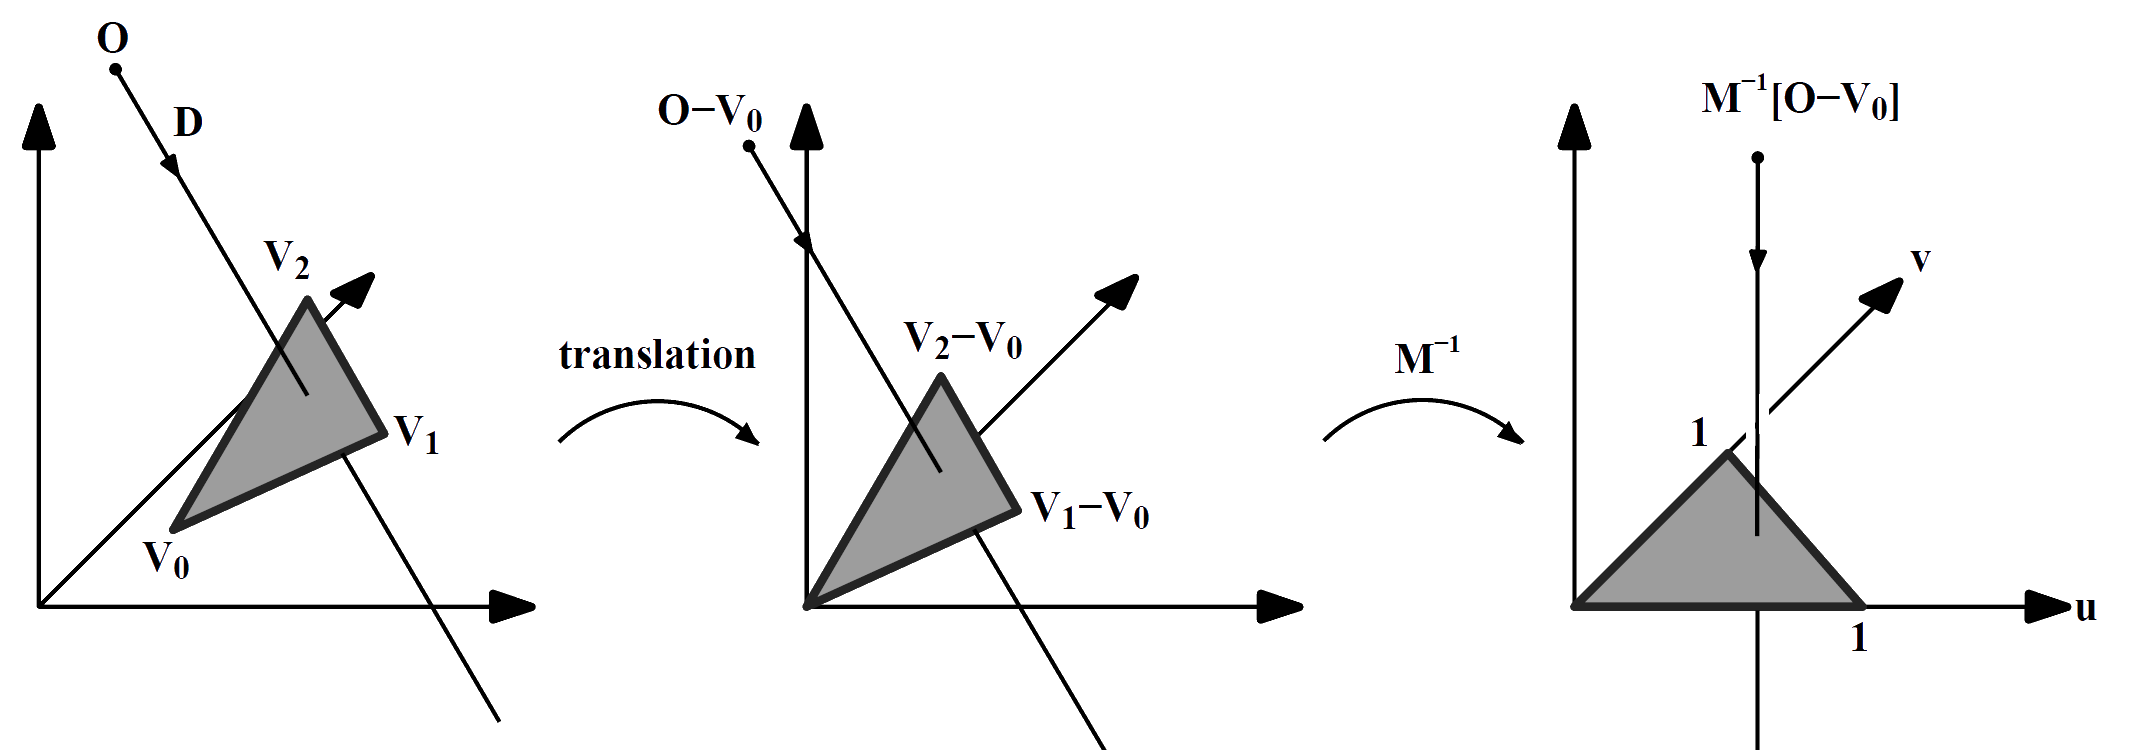
\includegraphics[width=0.9\textwidth]{moeller_trumbore}
	\begin{equation*}
		\left[-D, V_1 - V_0, V_2 - V_0 \right] \left[ \begin{array}{c} t \\ u \\ v \end{array} \right] = O - V_0
	\end{equation*}
	\caption{
		Principle of the famous Möller-Trumbore ray-triangle intersection test \cite{enlight_demo_workshop}.
	}
	\label{fig:ray_triangle_intersect}
\end{figure}
%
The intersection test relies on the idea that with a simple transformation, the problem can be represented in a coordinate system where the solution is almost given.
This transformation should put the origin of the coordinate system at one vertex of the triangle.
The axes of the new system are the two triangle edges as well as the inverted ray direction.
If the problem is represented in this space, the ray's origin holds the values of the $u$ and $v$ barycentric coordinate of the intersection point on the triangle as well as the distance $t$ of the triangle to the origin in multiples of the ray direction vector's length.
$u$ and $v$ are used to test whether the intersection point lies within the triangle and $t$ can be used as parameter in the line equation of the ray, $X = O + D \cdot t$, to retrieve the point of intersection.
The transformation necessary consists of two steps.
The first is a translation of $O$ by $-V_0$ to move the coordinate system's origin to a triangle vertex.
The second step is a change of basis with $\left[-D, V_1 - V_0, V_2 - V_0 \right]$ as base matrix.
This is done by multiplying with the inverse base matrix.
The result vector $\left[ t,  u,  v \right]$ then contains the desired values.
By moving the multiplication with the inversed base matrix to the other side, the equation in figure \ref{fig:ray_triangle_intersect} is obtained.
Möller and Trumbore solve this system of equations in matrix form using Cramer's rule and by calculating the determinant of a matrix using a cross and a dot product.
This allows to calculate the values of the solution vector incrementally to allow early exits.


\subsection{Numeric improvements}
\label{sec:numeric_improvements}

If the method described in this chapter would be tested on various scenes now, it would barely work for not even modest scenarios.
The problem is mainly numeric instability and the iterative nature of the approach.
Each calculation with a fixed precision is effected by small rounding errors when the result is stored back into a register or to memory.
This especially becomes a problem when theoretically equal calculations should practically yield equal results.
When two incident triangles for example intersect with a third triangle, the shared edge of the first two triangles should intersect at the same point on triangle three.
Depending on the order of operations this is not guaranteed.
The result may be different if, \eg, the two points representing the edge are swapped.
%
The triangle splitting algorithm for example can only hold its guarantees if the intersecting edges are true polylines with no gaps between the segments and their ends are exactly at the triangle edges.
Otherwise, degenerated triangles may be created between intersecting edges or at the triangle edges.
%
Another problem are algorithms which create very small numbers in intermediary calculations.
If a triangle is really thin, the dot product between the edges at the smallest corner is almost zero and might suffer severely from numerics.
The cross product and therefore the normal vector also becomes instable.
Calculations depending on these values might then critically misjudge a situation and \eg create intersection lines outside a triangle or falsely report a triangle as inside-a-structure based on a degenerated normal.
The problem with errors on such hard decisions is that they escalate with the number of iterations, which might be several hundreds or thousands.
If two structures are united but a wrongly discarded triangle left a hole, all following inside tests are affected and may fail.
Several improvements to mitigate degeneration and numeric errors are discussed in this section.

\begin{description}
	% TODO: add drawings
	
	\item[Collapse near points in structures] \hfill \\
	At the beginning of the \textproc{UnionStructure} algorithm almost no guarantees are given on the two input structures.
	As very thin or degenerated triangles are numerically problematic during the following algorithmic steps, \eg intersection, inside test, \etc, filtering them may avoid some of those problems.
	Therefore, all vertices which are closer than a defined small epsilon distance are collapsed to their mean.
	Thus, no holes are created in the structure, only degenerated triangles.
	These are easy to filter in a post-processing step by removing all triangles where two or more vertices are equal.
	

	\item[Flush tiny values to zero] \hfill \\
	Floating point values with tiny exponents, \eg $10^{-15}$ and below, tend to make some calculations unstable, especially when collapsing vertices with such coordinates.
	Collapsed vertices with such values might still not compare equal afterwards which breaks subsequent calls to the CDT algorithm.
	The reason therefore is unfortunately not clear.
	However, flushing such small values to zero eliminates the problem.
	
	
	\item[Verify intersection line] \hfill \\
	In situations where two triangles are quite thin, the Möller-Trumbore intersection test may report an intersection and calculate an intersection line which lies outside one or both of the triangles.
	Subsequent CDTs will then generate additional triangles outside the triangle which should be split as CDT routines usually triangulate the convex hull of the input point set.
	This issue is avoided by an additional test run after the call to \textproc{IntersectTriangles}.
	If a triangle intersection is recorded, test each point of the line if it lies on each of the triangles using a raycast with the point as origin and each triangle normal as ray direction.
	Only if the resulting $u$ and $v$ coordinates for both points are within their bounds including a small epsilon, \ie $-\epsilon \leq u \leq 1+\epsilon \wedge -\epsilon \leq v \leq 1+\epsilon \wedge u + v \leq 1 + \epsilon$, the intersection is accepted.
	
	
	\item[Collapse constraint vertices with structure vertices] \hfill \\
	Some of the intersection lines on a triangle might be very close to the triangle's vertices.
	To avoid creating degenerated triangles during CDT, all constraints' vertices are checked against the triangle's vertices to ensure a minimum distance.
	If a distance is less than a specified minimum, the affected vertex is set to the corresponding vertex of the triangle.
	
	
	\item[Collapse near points in constraints per triangle] \hfill \\
	This correction is the most important one.
	After all intersection lines have been recorded, collapse all constraint vertices which are closer than a defined epsilon distance.
	This routine ensures that each pair of incident triangles intersecting another triangle produce an incident pair of constraints.
	In other words, constrained edges which are not connected to each other because of numerical issues in the intersection routine are rejoined again to form closed polylines.
	Furthermore, tiny constraints collapse to points and are removed.
	This matter is important for correct splittings after running the CDT.
	
	
	\item[Ensure unique constraints] \hfill \\
	Constraint uniqueness is a small and simple check.
	The test is required as duplicated constraints impose a problem for some CDT libraries.
	
	
	\item[Specify hull constraints] \hfill \\
	Most CDT libraries triangulate a given point cloud within the convex hull of the cloud.
	Identifying the edges belonging to the convex hull is usually deterministic if the points are in what is called general position, \ie no coincident or collinear points.
	However, the vertices of a triangle and a set of constraints where many constraints end at the triangle's edges contain a lot of collinear points.
	To order to help the CDT in finding the right hull, it is recommended to specify the hull manually via additional constraints.
	These hull constraints are constructed from the triangle's vertices and the constraint vertices touching an edge of the triangle.
	The latter are identified by counting the number of constraints incident to each vertex of a point set formed by all constraints' vertices.
	Vertices with only one incident constraint must lie at the triangle's border and are therefore hull vertices.
	Together with the triangle's vertices, the hull vertices are ordered cyclical around their center of mass.
	The hull constraints are then formed from each adjacent pair of the ordered hull vertices including the constraint from the last to the first hull vertex.
	These hull constraints are appended to the constraints created by the intersection lines as input to the CDT.
	
	
	\item[Remove degenerate triangles after CDT] \hfill \\
	Despite good preparation of the input, it might still be the case that tiny or degenerated triangles are generated by the CDT routine, especially along the hull.
	The vertices of such triangles are apart far enough to pass vertex collapse in a following iteration.
	A check on the triangle's angles is therefore preferred.
	If the dot product of any pair of incident, normalized edges of the triangle is approaching zero, \ie is below a defined epsilon, the triangle is removed from the triangulation result.
\end{description}


\subsection{Parallelization}
\label{sec:parallelization}

By choosing to solve the intersections of all structures per cell, the main routine in algorithm \ref{alg:direct_intersection} became embarrassingly parallel.
As the regular grid usually consists of a larger number of cells, \eg $100 \times 100 \times 100$ is quite common, scheduling each cell in parallel is probably the best option for parallelization.
However, a good scheduling strategy is needed as the workload per cell is highly diverse.
Most of the cells are empty because they are either inside or outside cells and require no processing.
But also the amount of triangles and structures in each surface cell varies drastically between a few triangles and several thousands.

If all structures would be closed, \ie triangle elimination by classification would be disabled, and there would be no subdivision into cells, the iterative creation of the union structure could be parallelized instead.
Always combining two elements of a set of elements until only one left is an algorithm known as reduction, fold or accumulate.
Reductions are usually parallelized as tree.
Each independent pair of elements can be reduced into one in parallel.
However, tree-shaped parallel reduction offers suboptimal parallelism, especially against the end where only a few parallel pairs remain.
Parallelizing the reduction of all surfaces into one in addition to a cell-based parallelization is probably superfluous as the still high number of surface cells provide enough parallel work to saturate most workstation or even server CPUs.

Most routines inside the \textproc{UnionStructure} algorithm are also viable candidates for parallelization, although the workload is significantly smaller.
A structure inside a cell usually does not consist of more than 50 - 100 triangles.
These routines would probably benefit from data parallelism and SIMD constructs, \ie vectorization.
Especially the \textproc{ClipPolygonAABB}, \textproc{IntersectTriangles} and \textproc{IsTriangleInsideStructure} algorithms contain only a few branches and operate on simple data structures, \ie arrays.

Considering alternative hardware architectures like GPUs or similar accelerators, \eg Intel's Xeon Phi coprocessor, a parallelization based on the regular grid's cells is recommended.
The reason is that the number of cells is known at the beginning of the whole calculation which allows static scheduling of the entire work size.
This property is mandatory when programming for GPUs, but has been softened in recent years by the introduction of dynamic parallelism in CUDA 5.0 and OpenCL 2.0.
Furthermore, as most GPU architectures rely on either vectorization or execution of thread groups in lockstep\footnote{
	Most GPUs usually schedule groups of threads, called warps with 32 threads by NVIDA and wavefronts with 64 threads by AMD.
	These threads are tied together and executed instruction-wise, meaning all threads execute the same instruction on their individual data in parallel.
	This behavior is also called lockstep execution.
	If some threads branch differently than others, \eg if, while or for statements, all threads execute both branches, but some of them are masked out to avoid changes by the executed instructions.
	Intel's on-chip GPUs rely on vectorization which has to be done manually by the programmer for medium and advanced algorithms.},
the uneven work loads in all loops, \eg number of structures per cell, number of triangles per structure, number of intersections, \etc, especially hurt these architectures, probably causing many threads to run empty loops because of a few larger cells or structures.


\section{Test scenes}
\label{sec:test_scenes}

For testing the direct intersection approach and the further surface reconstruction algorithms shown in succeeding chapters, a few test scenes have been created.
The test scenes and their configurations are shown in table \ref{tbl:test_scenes}.
%
\begin{table}[h]
	\centering
	\begin{tabular}{lrrrrrrrr}
		Scene          & SVs  & cells & surf. & tri. & tri./SV & s\textsubscript{max} & s\textsubscript{avg} \\
		\hline
		cube2          &    1 &   1k & 47 \% &   0.8k &  2 & 1.1 \\
		cylinders\_d   &    1 &   1k & 22 \% &     7k &  2 & 1.1 \\
		cylinders      &    1 &   1k & 22 \% &     4k &  2 & 1.1 \\
		cylinder\_head &   20 &  75k & 21 \% &    80k &  3 & 1.2 \\
		impeller       & 2383 & 400k & 16 \% &  6000k & 64 & 5.5 \\
		impeller\_2    & 1191 & 400k & 13 \% &  3000k & 64 & 3.6 \\
		turbine        &  480 & 200k & 17 \% & 16000k &  6 & 2.3 \\
	\end{tabular}
	\caption{
		Table containing the selected test scenes and several parameters of them.
		It lists the name of a scene, the number of swept volumes, the total number of cells of the regular grid, the amount of surface cells in the grid, \ie cells which have to be processed, the total amount of triangles in the grid as well as the maximum and average amount of structures in a cell.
	}
	\label{tbl:test_scenes}
\end{table}

The cube2 scene is a simple intersection between a cubic stock and a cuboid swept volume.
It has already been used as an example when discussing the concept of the direct intersection approach at the beginning of this chapter in figure \ref{fig:cube2}.
But instead of no grid, a small one with a resolution of $10\times10\times10$ cells is used.
This scene is used as a proof of concept for each surface reconstruction algorithm in this thesis.
%
The cylinders and cylinders\_d scenes each consist of a broader cylindrical stock with a smaller cylindrical swept volume drilled out.
The cylinders in the cylinders\_d scene are triangulated into smaller and more regular triangles by constraining the edge lengths of the output triangles.
The cylinders in the other scene contain longer and thiner triangles.
The cylinders\_d scene requires more triangles to approximate the cylinders 
Both scenes also use the same small grid resolution as the cube2 scene.
These two scenes should have an almost identical visual outcome but quite different stress on the numeric robustness of the extraction.
%
The cylinder\_head scene was the initial test scene when the ray casting subsystem was developed, \cf chapter \ref{ch:previous_work}.
It is the smallest and easiest of the practical scenes used for benchmarking.
The cylinder\_head uses a medium sized grid of $50\times50\times30$ cells with a moderate, but still little, number of triangles and swept volumes.
%
The impeller scene provide a good real world example of a typical machining scenario.
It contains a few thousand swept volumes organized in a larger grid of $100\times100\times40$ cells.
With 6 million stored triangles and a lot more structures in each cell, the impeller scene should already pose a serious workload for the tested algorithms.
To analyze the effect of the number of swept volumes, a second version of the impeller scene has been created, where only half the number of swept volumes have been loaded.
%
Finally, the turbine scene depicts a further practical example.
The scene was initially conceived to stress the swept volume computation by its complex cutting tool, a fir-tree cutter.
The fine tessellation of the cutter mesh results in high resolution swept volumes and the largest amount of triangles stored in a test scene.

The amount of triangles in each grid cell varies greatly between the test scenes and also in the scenes themselves.
This property is interesting as it has the largest impact on algorithms which have to iterate on the triangles of a cell.
Furthermore, largely divergent triangle counts inside cells challenge schedulers in parallel processing of cells and increase branch divergence on GPU architectures.
An optimal distribution would be an almost empty histogram with a peak at a certain location, meaning all surface cell contain roughly the same number of triangles.
Figure \ref{fig:histograms} shows histograms of the triangles per cell distribution for the test scenes of table \ref{tbl:test_scenes}.
%
\begin{figure}[!]
	\centering
	\begin{subfigure}[b]{0.49\textwidth}
		\centering
		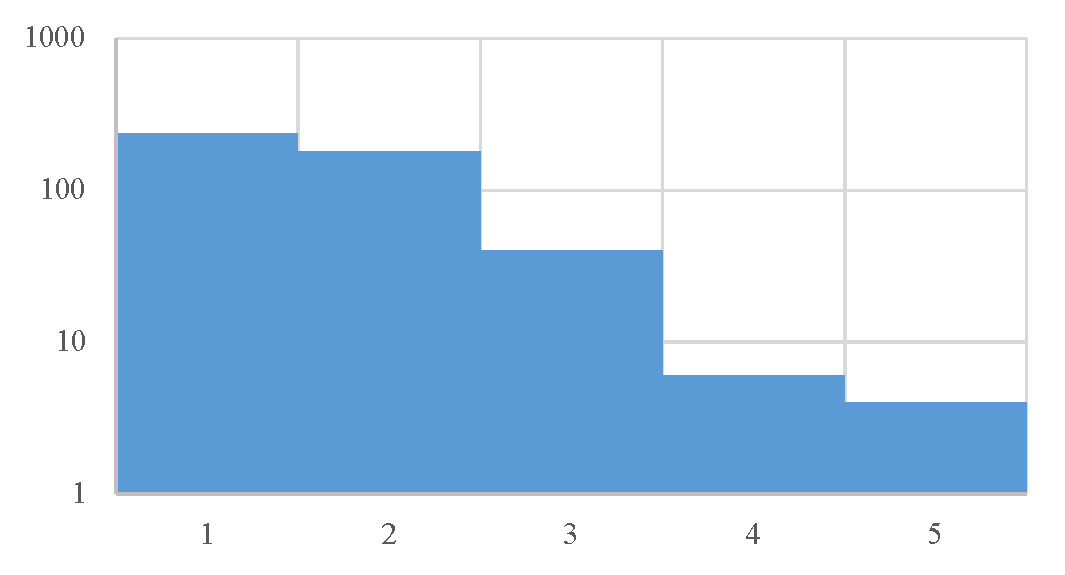
\includegraphics[width=\textwidth]{c_hist}
		\caption{cube2}
		\label{fig:cube2_histogram}
	\end{subfigure}
	\begin{subfigure}[b]{0.49\textwidth}
		\centering
		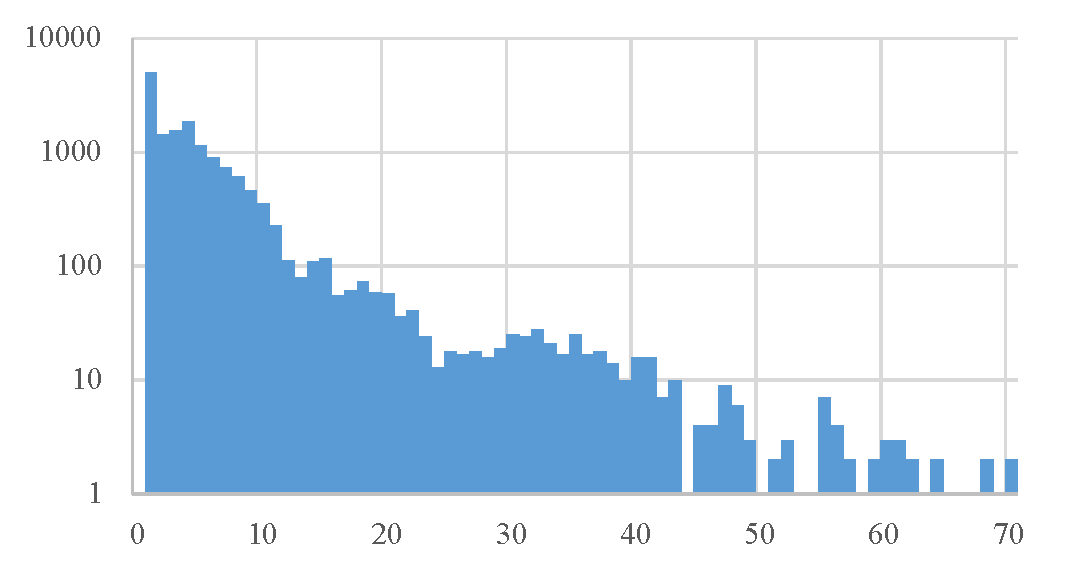
\includegraphics[width=\textwidth]{ch_hist}
		\caption{cylinder\_head}
		\label{fig:cylinder_head_histogram}
	\end{subfigure}
	\begin{subfigure}[b]{0.49\textwidth}
		\centering
		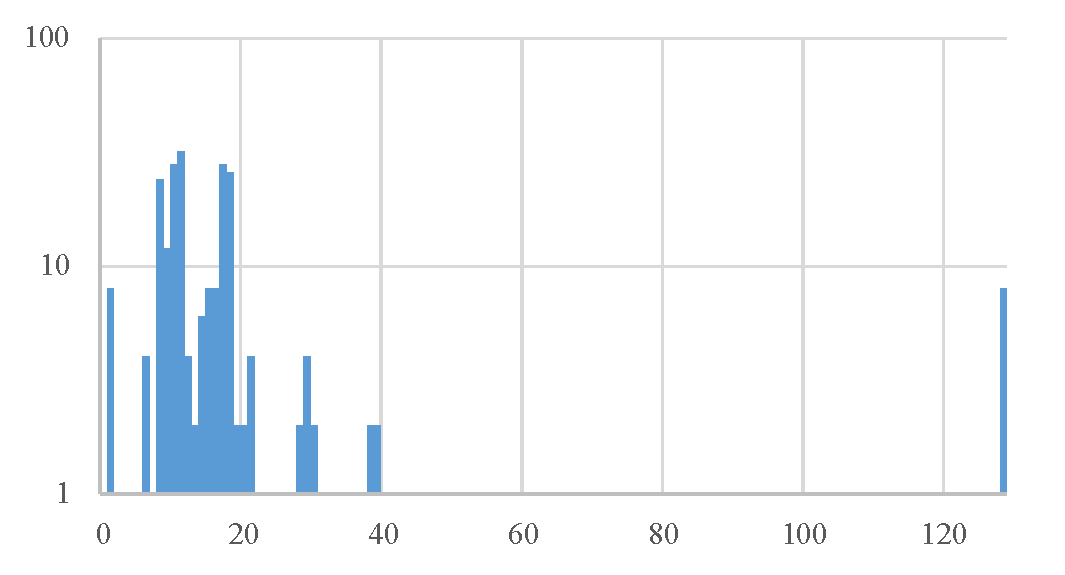
\includegraphics[width=\textwidth]{cy_hist}
		\caption{cylinders}
		\label{fig:cylinders_histogram}
	\end{subfigure}
	\begin{subfigure}[b]{0.49\textwidth}
		\centering
		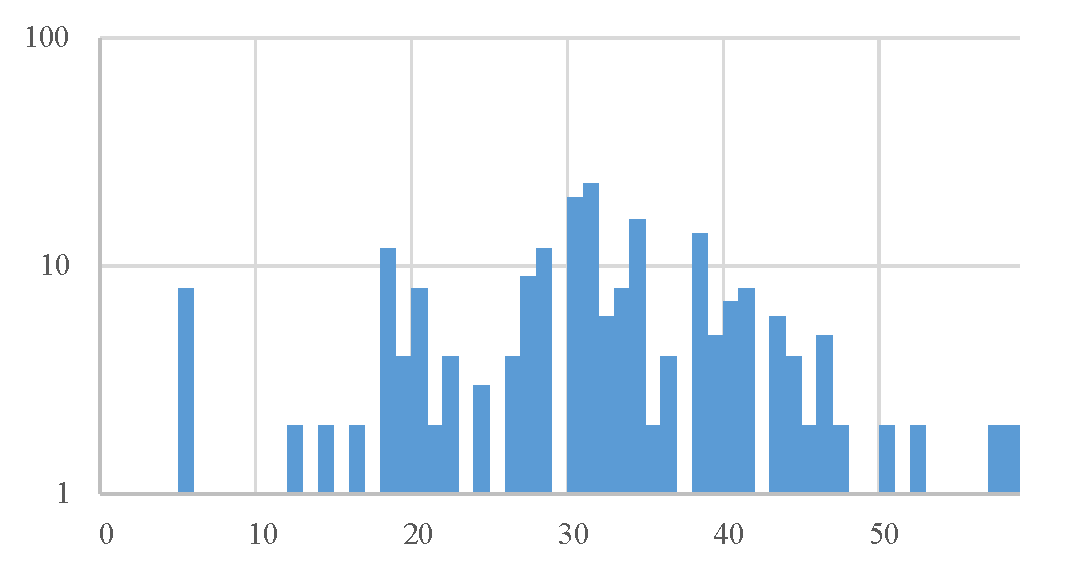
\includegraphics[width=\textwidth]{cyd_hist}
		\caption{cylinders\_d}
		\label{fig:cylinders_d_histogram}
	\end{subfigure}
	\begin{subfigure}[b]{0.49\textwidth}
		\centering
		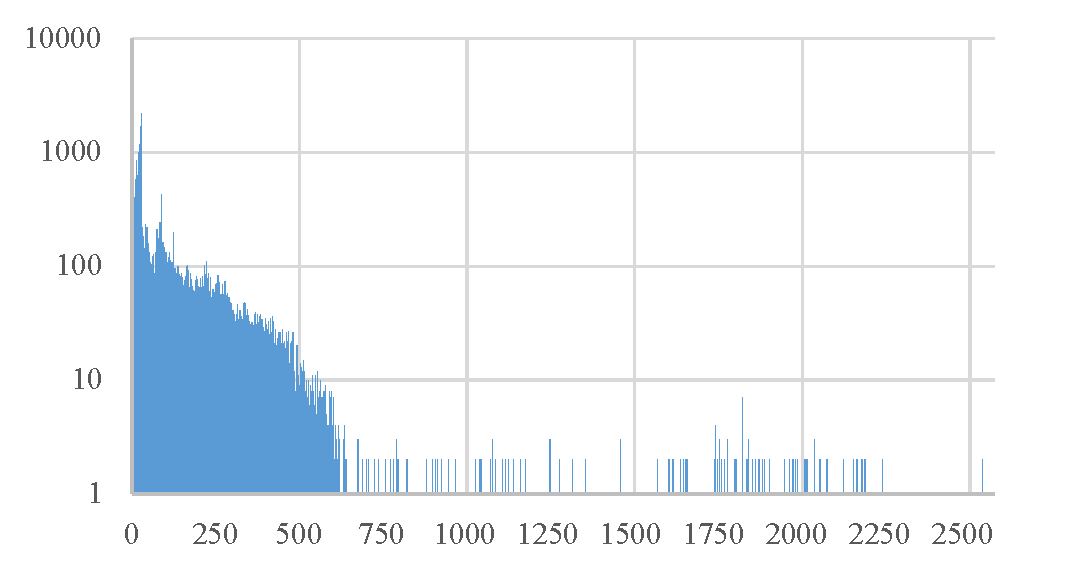
\includegraphics[width=\textwidth]{hq_hist}
		\caption{impeller}
		\label{fig:impeller_histogram}
	\end{subfigure}
	\begin{subfigure}[b]{0.49\textwidth}
		\centering
		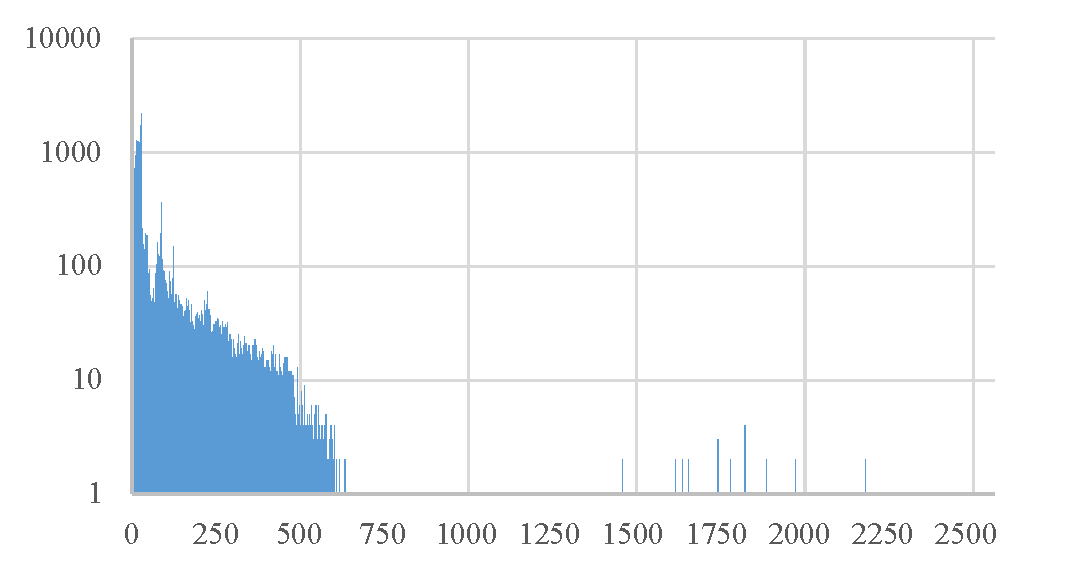
\includegraphics[width=\textwidth]{hq2_hist}
		\caption{impeller\_2}
		\label{fig:impeller_2_histogram}
	\end{subfigure}
	\begin{subfigure}[b]{0.49\textwidth}
		\centering
		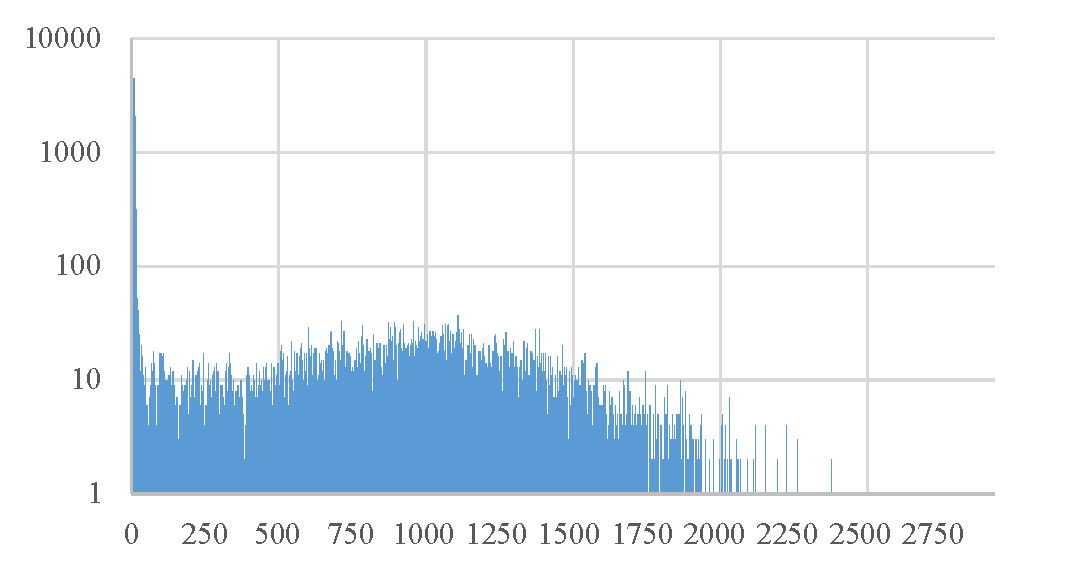
\includegraphics[width=\textwidth]{tr_hist}
		\caption{turbine}
		\label{fig:turbine_histogram}
	\end{subfigure}
	\caption{
		Histograms showing the distribution of triangle counts per cell for the selected test scenes in table \ref{tbl:test_scenes}.
		The horizontal axis shows the number of triangles per cell.
		The vertical axis is logarithmic and shows the number of cells with a specific triangle count.
	}
	\label{fig:histograms}
\end{figure}
%
The cube2 scene contains few triangles in general.
Most cells contain only 1 or 2 triangles and probably not more than 1 structure.
Larger cells contain 4 or 5 triangles occur infrequent.
In general, the distribution is quite compact.
%
The cylinder\_head is characterized by a quite divergent distribution, although the range is still modest from many cells with a small triangle count to only a few cells with 40 to 70 triangles.
%
Considering the cylinders scenes, the histograms show the difference in the total number of triangles.
As the cylinders\_d scene contains more, smaller and more regular triangles, its cells are also occupied by more triangles.
Whereas the cylinders scene holds mostly between 5 and 20 triangles, the cylinders\_d scene's cells contain mostly between 20 and 45 triangles.
Nevertheless, despite their lower triangle counts, there is a peek of triangles in the cylinders scene at 128 triangles, which are cells at the cylinder's center.
%
The impeller scene shows a quite good but broad distribution with many cells containing between 1 and 100 triangles.
A further lot of cells then store up to around 500 triangles.
Unfortunately, the impeller scene contains several cells with extraordinary high quantities of triangles up to 2574 triangles in a single cell, 2563 for the impeller\_2 scene.
%
Finally, the turbine scene attracts attention by its smooth distribution of triangle counts.
Despite its uniformity, such distributions are unfortunately rather disadvantages as the workload per cell is highly diverse.
Furthermore, the triangle counts per cell are quite high with amounts of up to 2000 triangles per cell occurring quite often.
Cells with even more triangles exist only marginally.

For visual reference, figure \ref{fig:raycasted_scenes} shows images of the selected test scenes raycasted using the VML.
%
\begin{figure}[!]
	\centering
	\begin{subfigure}[b]{0.43\textwidth}
		\centering
		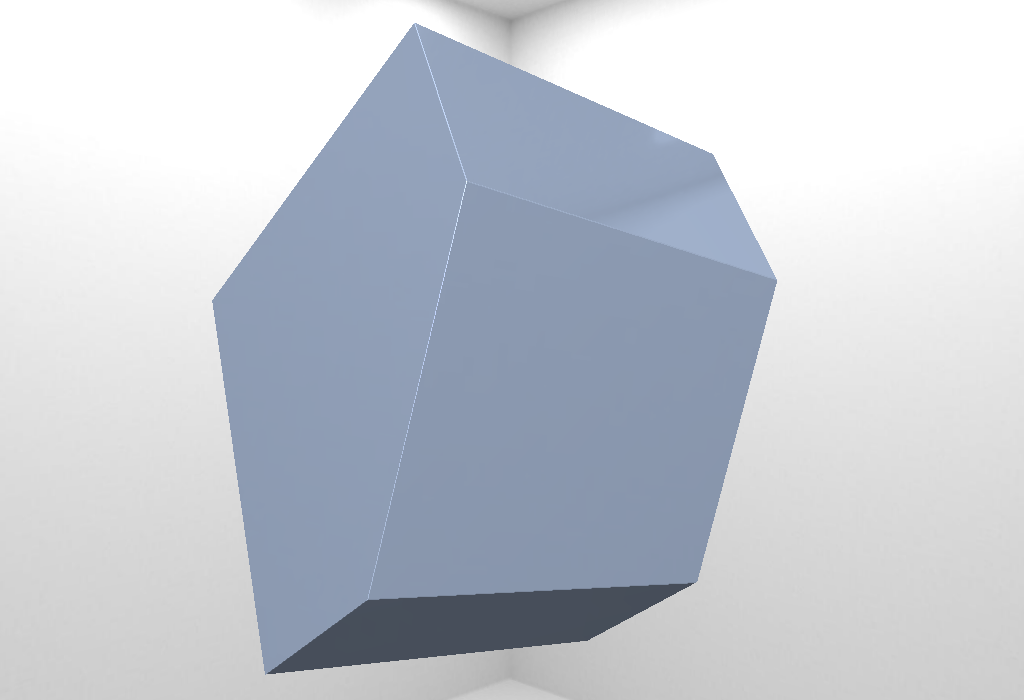
\includegraphics[width=\textwidth]{raycasted_cube2}
		\caption{cube2}
		\label{fig:cube2_raycasted}
	\end{subfigure}
	\begin{subfigure}[b]{0.43\textwidth}
		\centering
		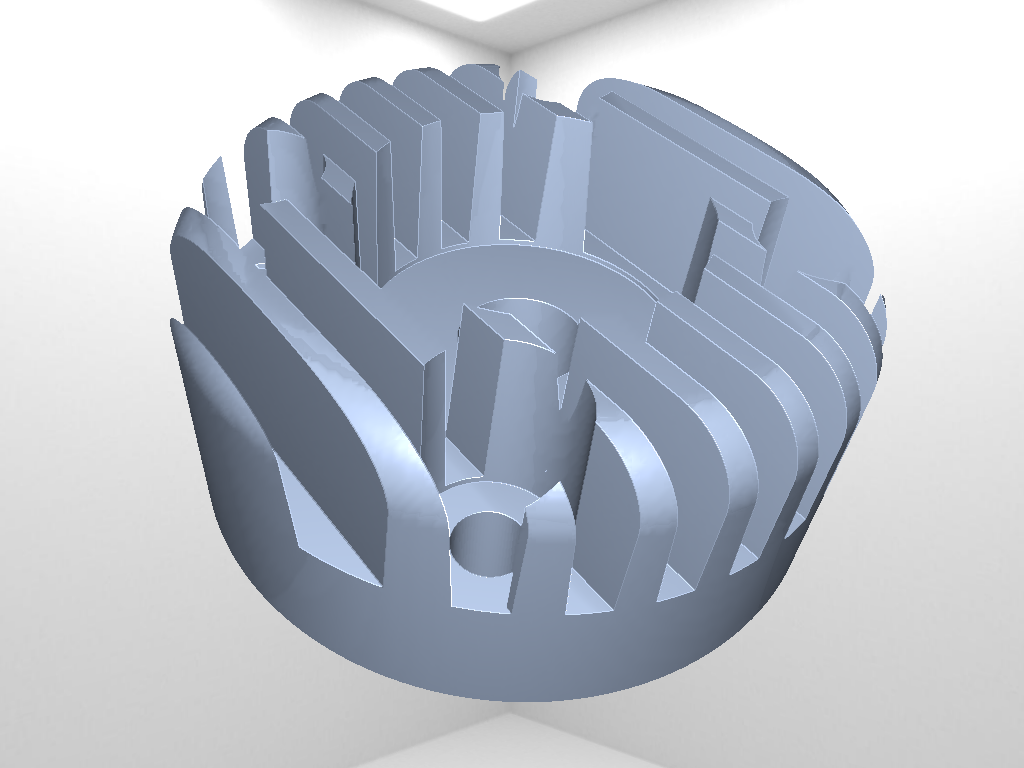
\includegraphics[width=\textwidth]{raycasted_cylinder_head}
		\caption{cylinder\_head}
		\label{fig:cylinder_head_raycasted}
	\end{subfigure}
	\begin{subfigure}[b]{0.43\textwidth}
		\centering
		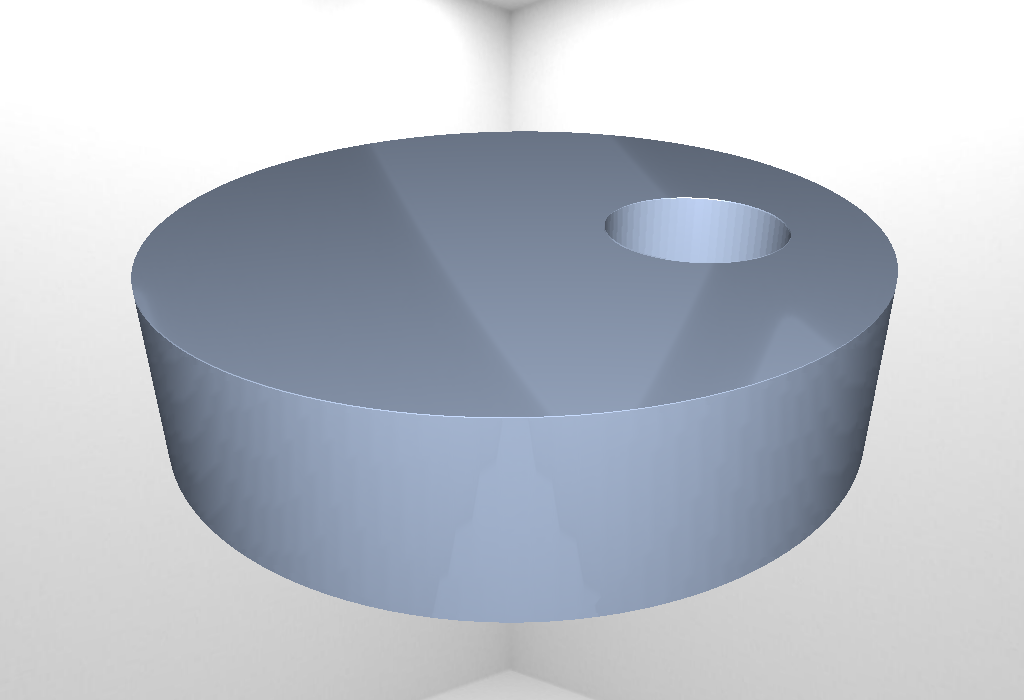
\includegraphics[width=\textwidth]{raycasted_cylinders}
		\caption{cylinders}
		\label{fig:cylinders_raycasted}
	\end{subfigure}
	\begin{subfigure}[b]{0.43\textwidth}
		\centering
		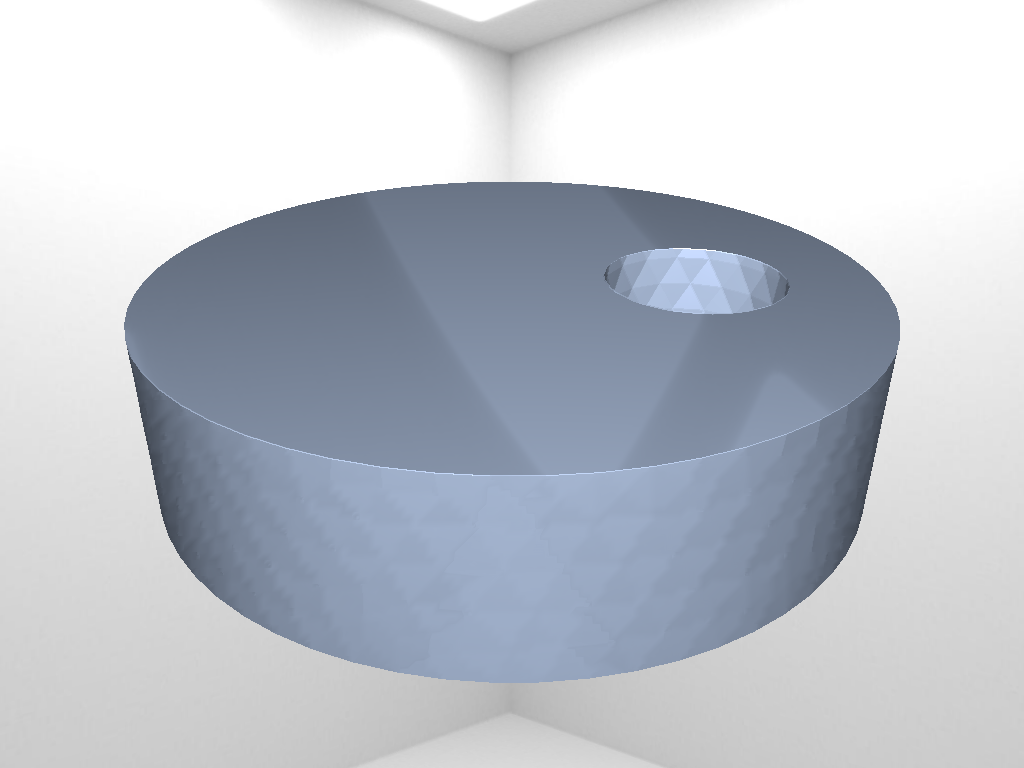
\includegraphics[width=\textwidth]{raycasted_cylinders_d}
		\caption{cylinders\_d}
		\label{fig:cylinders_d_raycasted}
	\end{subfigure}
	\begin{subfigure}[b]{0.43\textwidth}
		\centering
		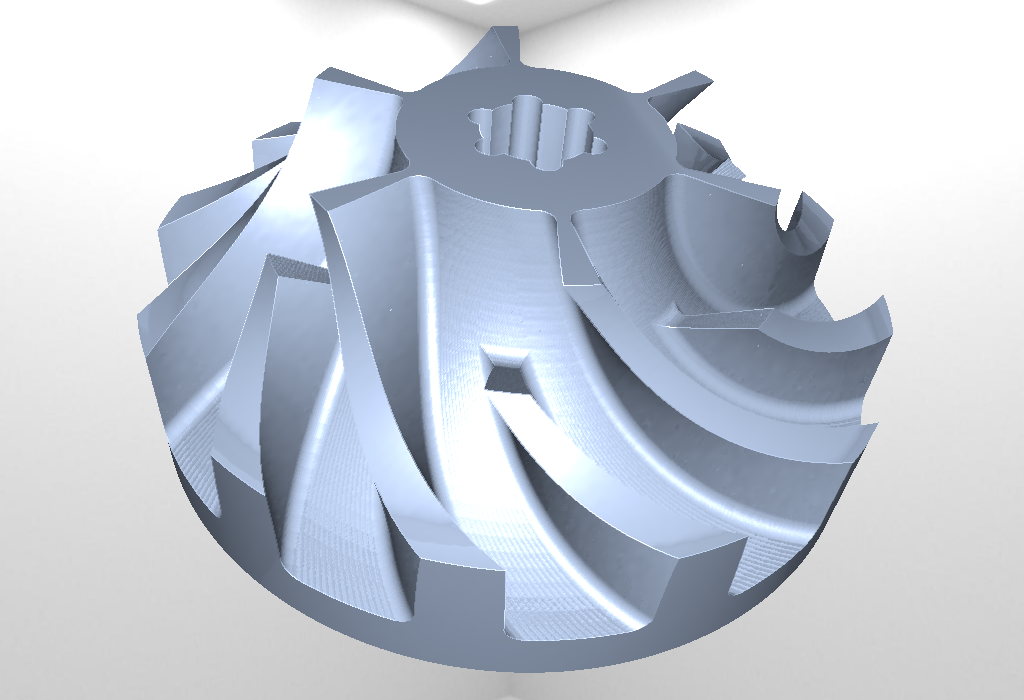
\includegraphics[width=\textwidth]{raycasted_impeller}
		\caption{impeller}
		\label{fig:impeller_raycasted}
	\end{subfigure}
	\begin{subfigure}[b]{0.43\textwidth}
		\centering
		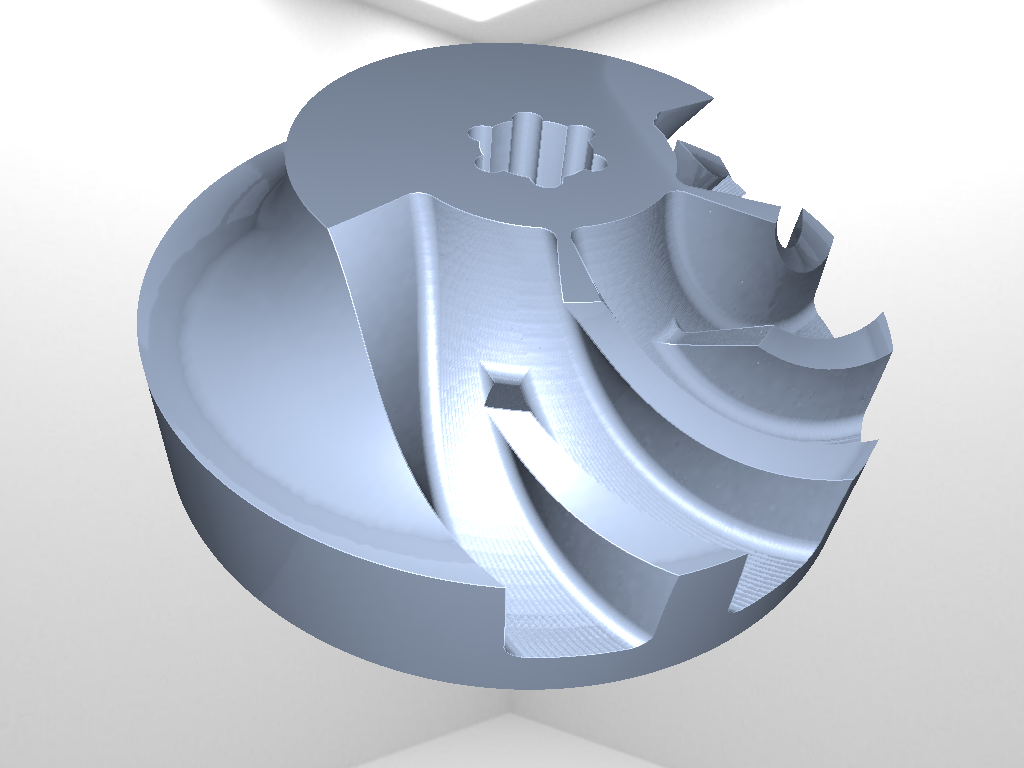
\includegraphics[width=\textwidth]{raycasted_impeller_2}
		\caption{impeller\_2}
		\label{fig:impeller_2_raycasted}
	\end{subfigure}
	\begin{subfigure}[b]{0.43\textwidth}
		\centering
		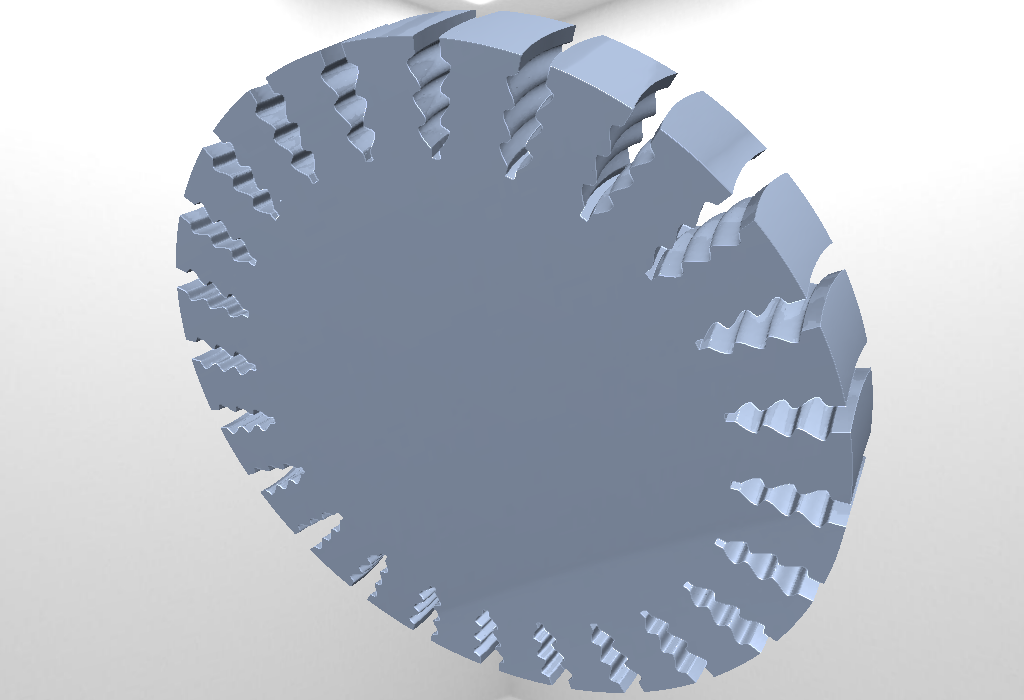
\includegraphics[width=\textwidth]{raycasted_turbine}
		\caption{turbine}
		\label{fig:turbine_raycasted}
	\end{subfigure}
	\caption{
		Raycasted images of the test scenes given in table \ref{tbl:test_scenes}.
	}
	\label{fig:raycasted_scenes}
\end{figure}

\section{Results}
\label{sec:direct_intersection_results}

Finally, the direct intersection approach described in this chapter has been tested on the scenes described in section \ref{sec:test_scenes}.
Table \ref{tbl:direct_intersection_results} contains the runtime and output size of the test runs.
%
\begin{table}[!]
	\centering
	\begin{tabular}{lrrrr}
		Scene          & SVs  & t\textsubscript{in} & t\textsubscript{out} & time \\
		\hline
		cube2          &    1 &   0.8k &    1k &   1ms \\
		cylinders\_d   &    1 &     7k &   10k &   6ms \\
		cylinders      &    1 &     4k &    7k &   9ms \\
		cylinder\_head &   20 &    80k &  149k & 229ms \\
		impeller       & 2383 &  6000k & 1677k &  21s  \\
		impeller\_2    & 1191 &  3000k & 1296k &  11s  \\
		turbine        &  480 & 16000k &  752k & 280s  \\
	\end{tabular}
	\caption{
		Test results for the direct intersection surface extraction approach.
		Runtime is averaged over 10 runs.
	}
	\label{tbl:direct_intersection_results}
\end{table}
%
The timings vary a lot from 1ms for the simple cube2 scene up to 280s for the turbine scene.
The runtime depends on multiple characteristics of the input.
The number of swept volumes increase the runtime linearly, as seen when comparing the timings of the impeller and impeller\_2 scene.
This consequence can also be derived from algorithm \ref{alg:direct_intersection} where the \textproc{DirectIntersection} function performs a pairwise reduction of all structures of a single cell, a linear operation.
All other parameters influence the runtime in less easily comprehensible ways.
The turbine scene for example has a little more than 3 times the triangles to process than the impeller scene and a lot less swept volumes, but requires more then 10 times the computation time.
What causes the big difference in this case is mostly the triangle density per structure.
When dividing the number of totally stored triangles by the number of swept volumes, we can get a rough idea of the complexity of a single swept volume.
This number is roughly 2500 for the impeller scenes and 33000 for the turbine scene.
As the grid resolution is almost identical in these scenes, the parts of a swept volumes assigned to each cell, \ie the structures, are substantially larger.
An increase in the number of triangles per structure, raises the runtime quadratically in several sub-algorithms.
Having a look on the basic structure of the direct intersection approach in algorithm \ref{alg:direct_intersection}, the \textproc{ClipStructure} and the \textproc{SplitTriangle} functions run linearly with the number of triangles per structure, whereas the \textproc{IntersectTriangle} and \textproc{IsTriangleInsideStructure} form nested loops on all triangles of the structure, \ie require quadratic time.
Considering the additional code required to increase numeric stability discussed in section \ref{sec:numeric_improvements}, the collapsing of near points of a structure is also a quadratic operation.
The algorithms with quadratic runtime also light up in profiling sessions with \textproc{IntersectTriangle} consuming 38\%, near points collapsing 26\% and \textproc{IsTriangleInsideStructure} 18\% of the total runtime.
The grid resolution affects the runtime by partitioning the whole problem into smaller parts.
A finer grid causes structures to be smaller and the output to contain fewer errors as cells contain fewer structures and triangles.
Especially the quadratic functions benefit from smaller structures.
However, as a consequence of a finer grid, more cells have to be processed in total.
As processing cells is a linear operation, \cf algorithm \ref{alg:direct_intersection}, increasing the grid resolution is usually beneficial.
Nevertheless, maintaining the grid and related data structures requires time and especially memory, thus restricting its granularity.
Resolutions between 100 and 150 cells in one dimensions usually proofed to be good choices for real world scenarios.

The amount of exploitable parallelism has already been discussed in section \ref{sec:parallelization}.
The topmost loop of the \textproc{DirectIntersection} function has been parallelized in the implementation using Microsoft's Parallel Patterns Library (PPL) and the parallel\_for function which uses a scheduler implementing work stealing to balance the workload \cite{ppl_parallel_for}.
The CPU utilization during an single run of the direct intersection approach on the impeller scene is shown in figure \ref{fig:di_cpu}.
%
\begin{figure}[!]
	\centering
	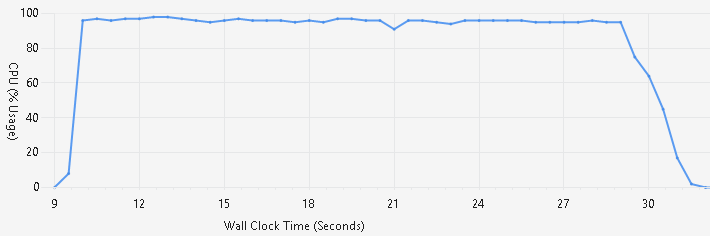
\includegraphics[width=0.8\textwidth]{di_hq_impeller_cpu}
	\caption{
		CPU utilization during a run of the direct intersection algorithm to reconstruct the surface of the impeller scene.
	}
	\label{fig:di_cpu}
\end{figure}
%
The CPU cores are almost perfectly utilized for the first 20 seconds.
Afterwards, the workload drops done to zero within the last 3 seconds of the run.
The PPL's default scheduler already does a pretty good job by keeping all cores utilized for 85\% of the runtime.
This slow drop at the end of the test run might be improved by employing a better scheduling strategy.
However, more complex scheduling usually also increases the parallelization overhead.
Concerning memory, the regular grid holding the impeller requires approximately 600 MiB memory.
During the algorithm, 300 MiB additional memory has been allocated, mostly for the temporary union structures and the buffer holding the resulting surface.

Figure \ref{fig:di_results} contains renderings of the resulting triangle meshes.
%
\begin{figure}[!]
	\centering
	\begin{subfigure}[b]{0.34\textwidth}
		\centering
		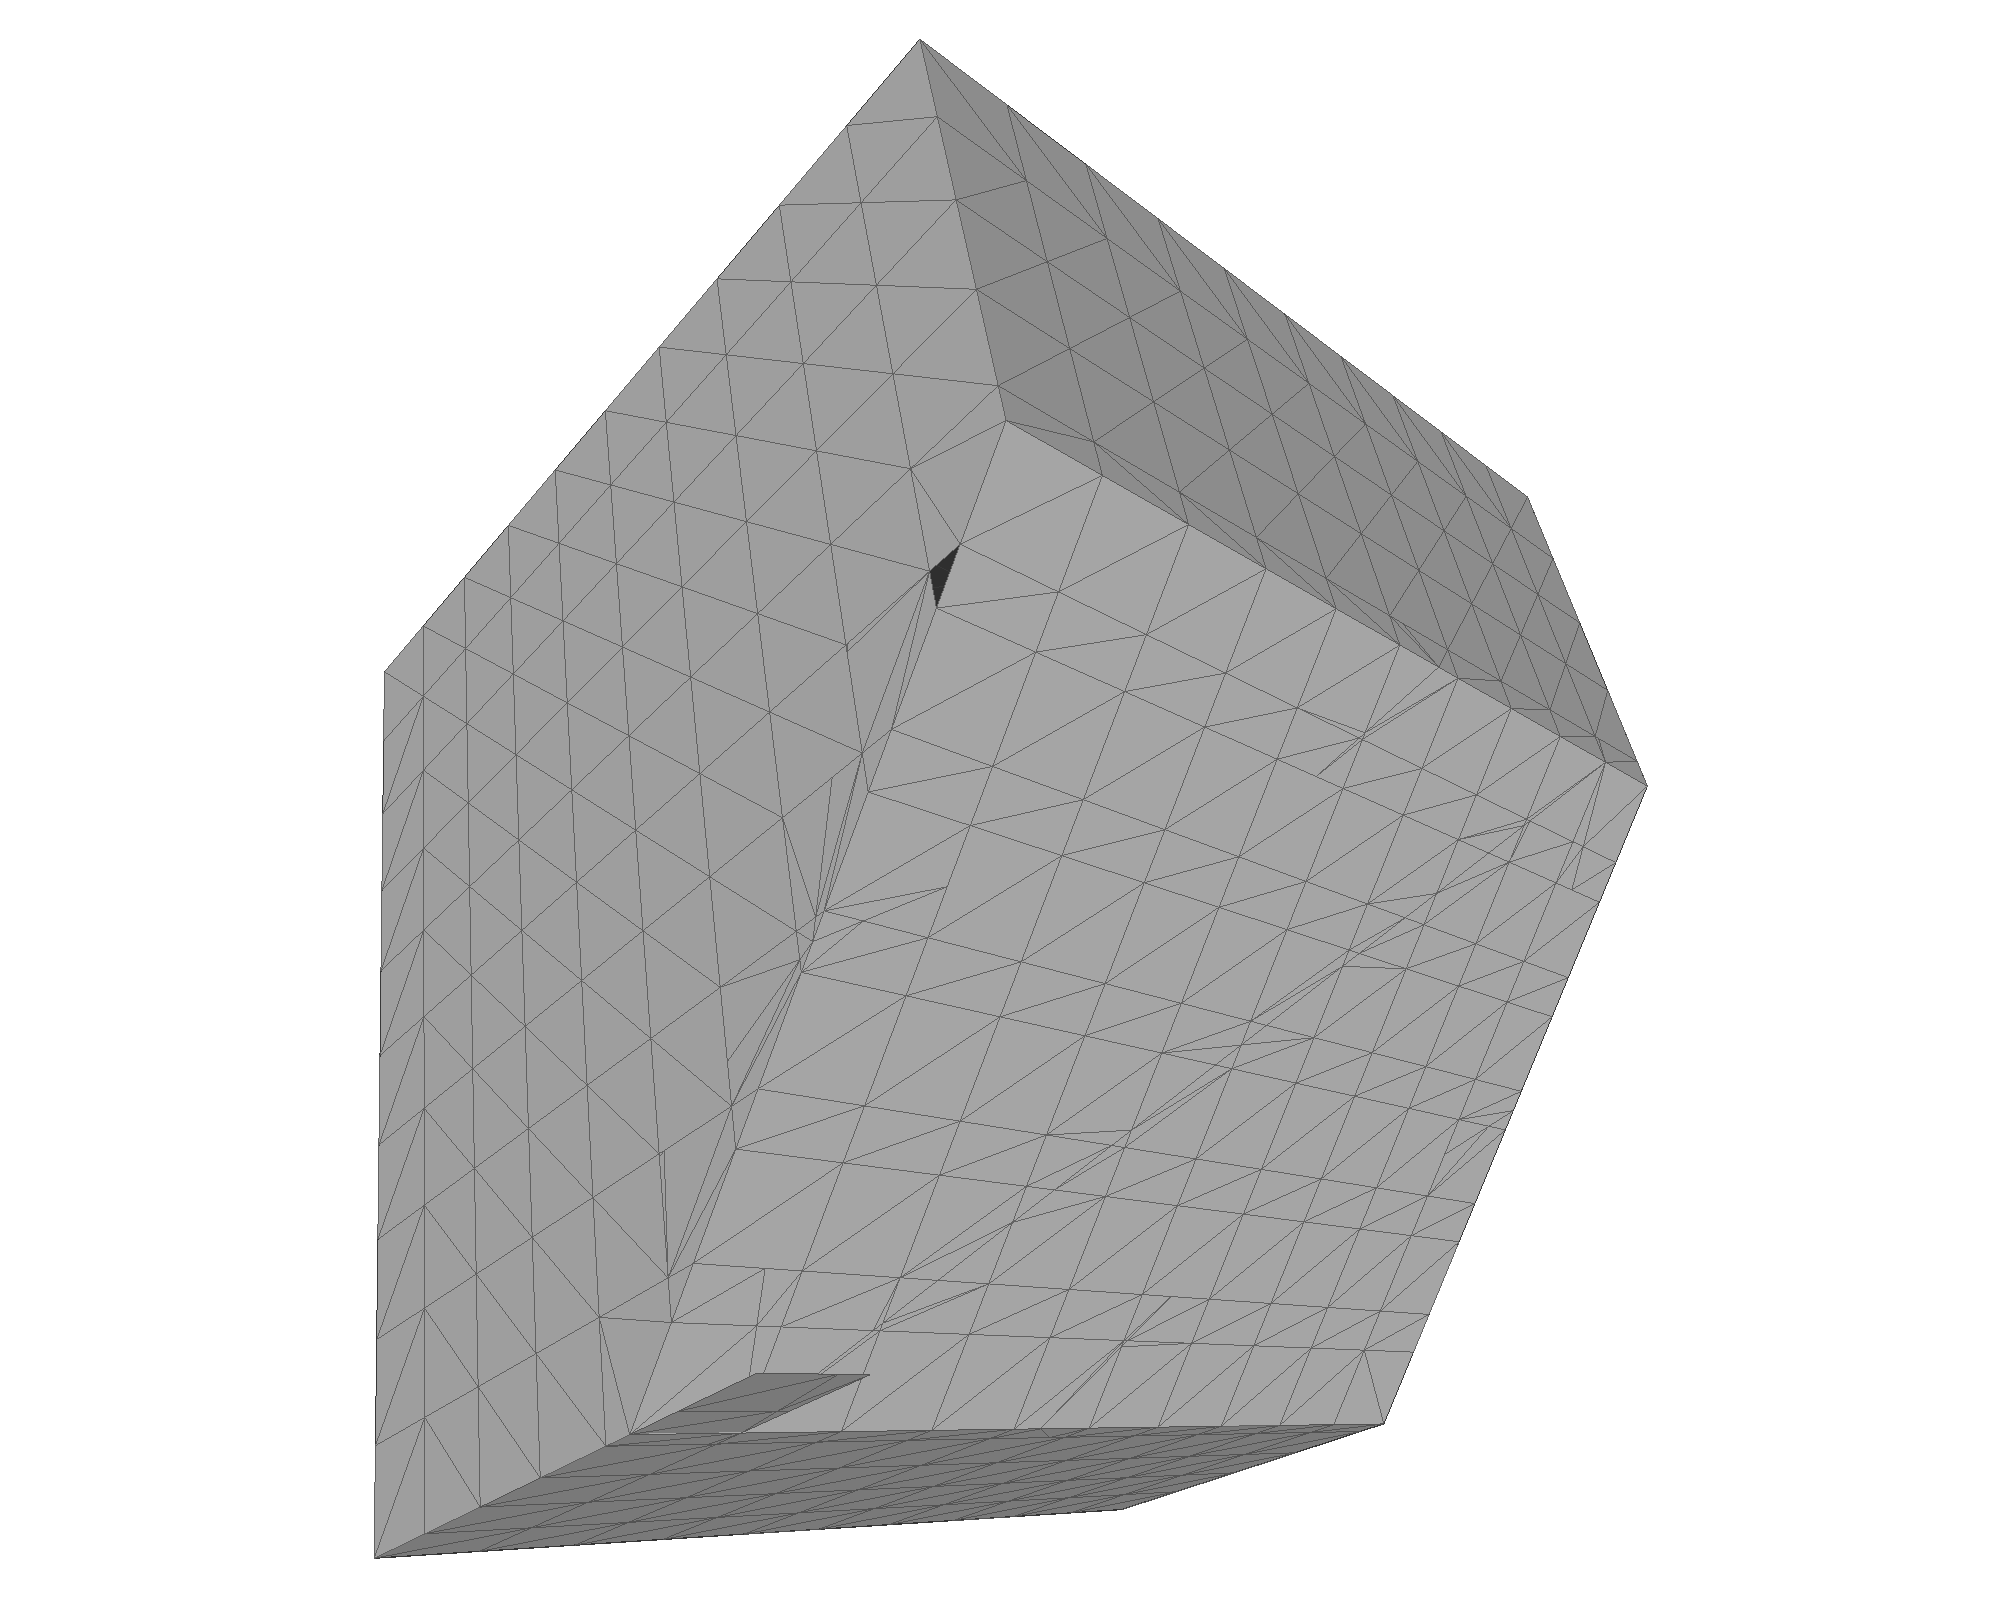
\includegraphics[width=\textwidth]{di_cube2}
		\caption{cube2}
		\label{fig:di_cube2}
	\end{subfigure}
	\hspace{1cm}
	\begin{subfigure}[b]{0.34\textwidth}
		\centering
		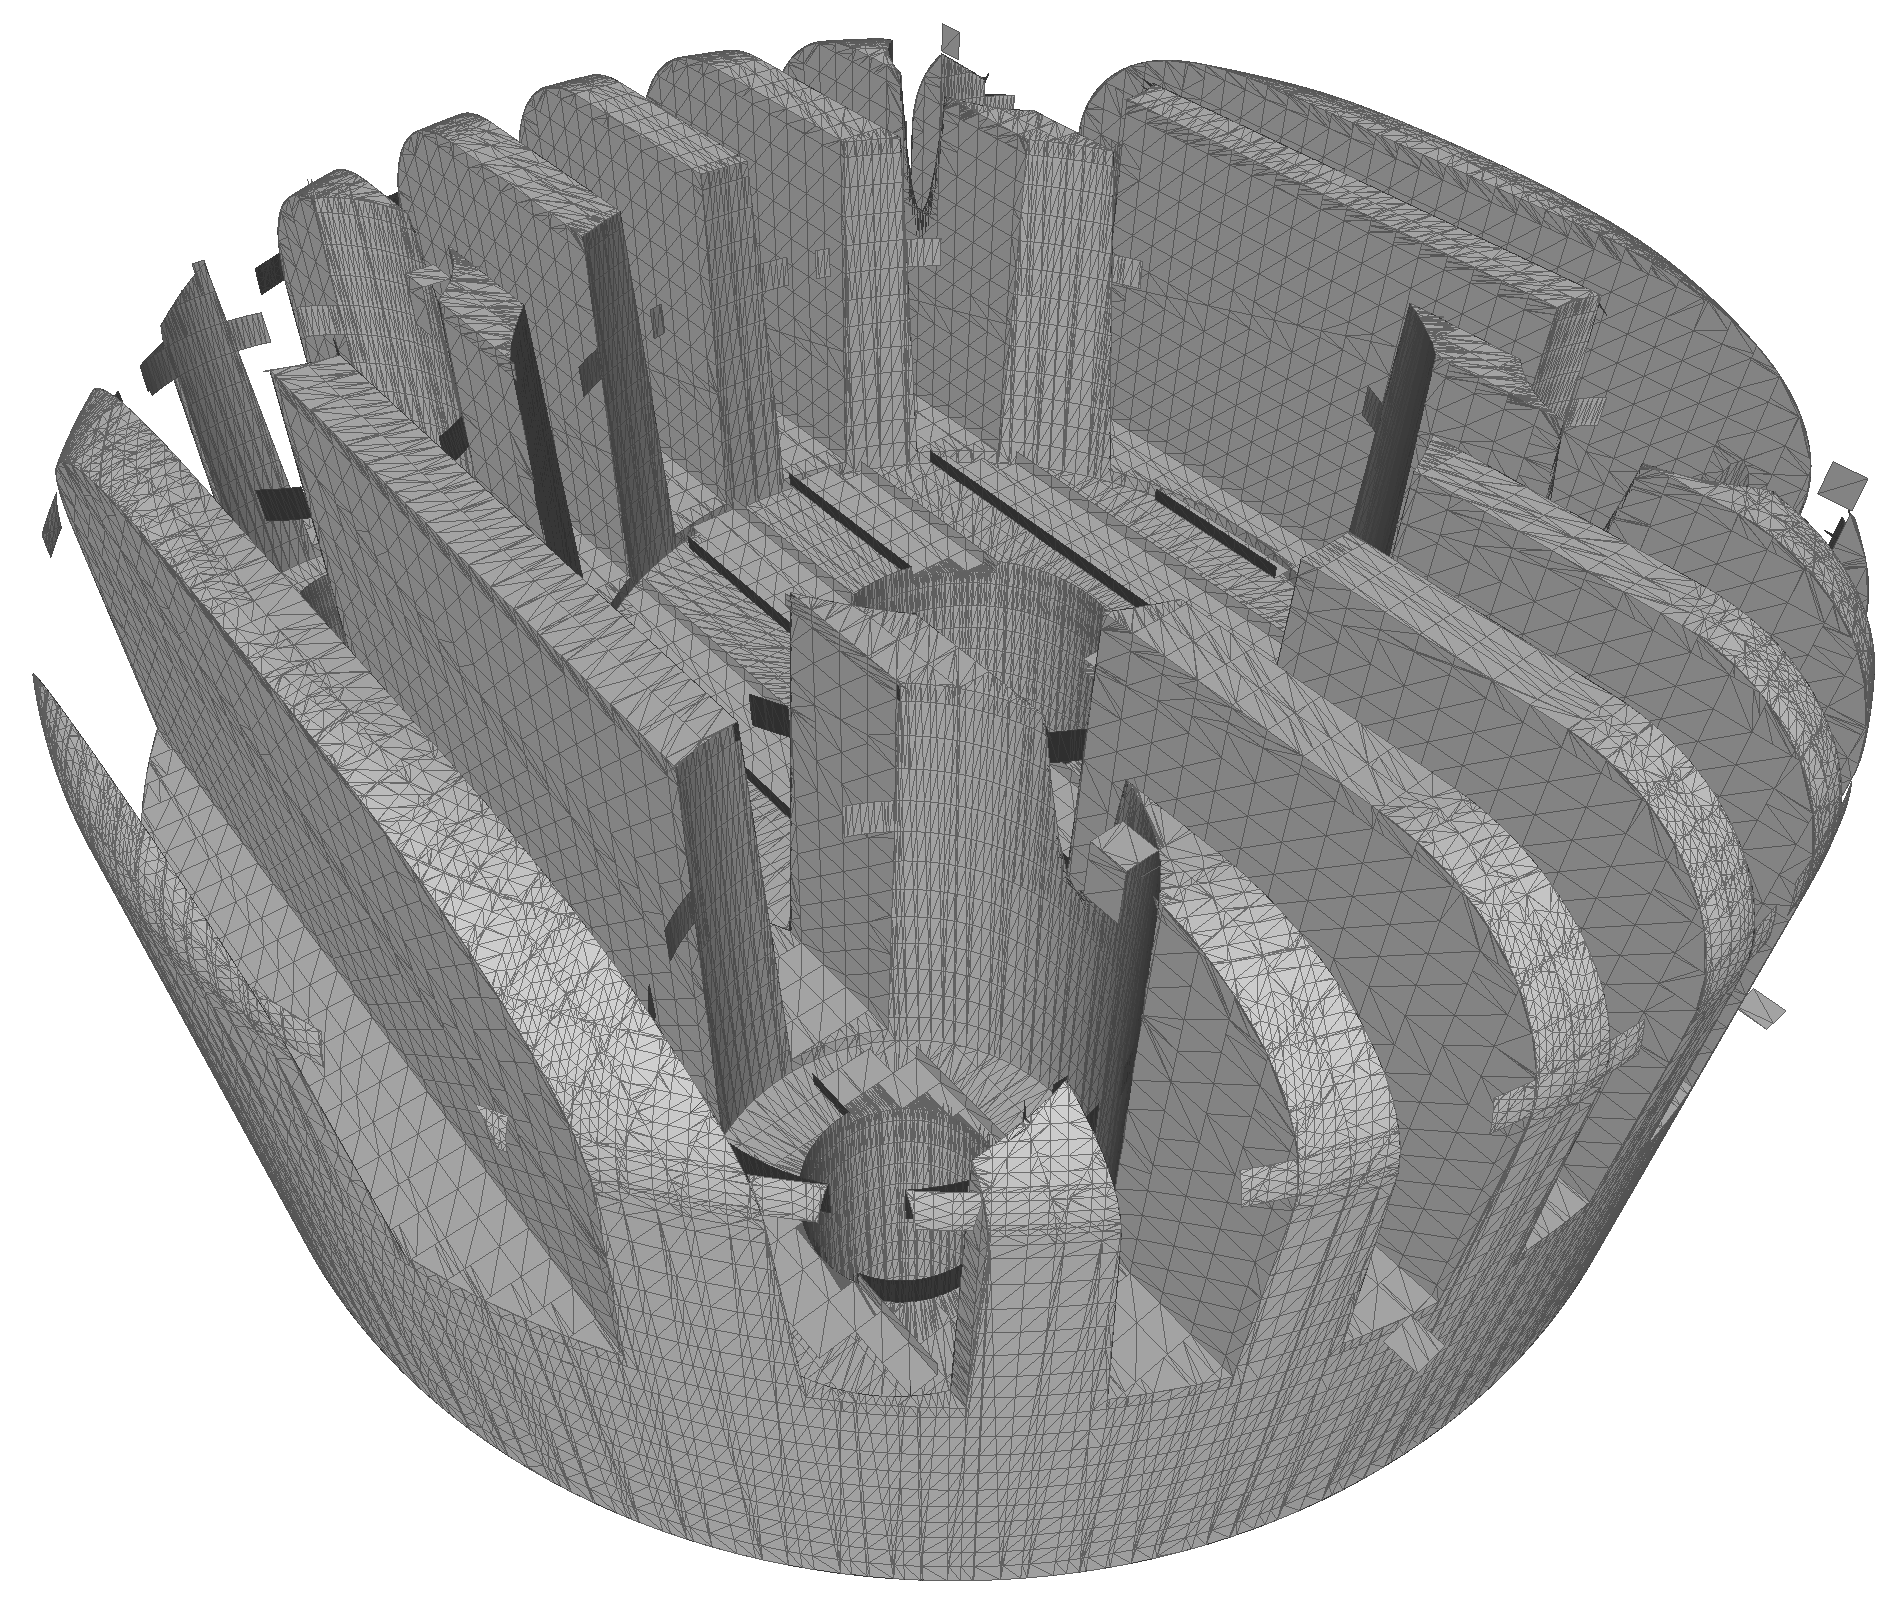
\includegraphics[width=\textwidth]{di_cylinder_head}
		\caption{cylinder\_head}
		\label{fig:di_cylinder_head}
	\end{subfigure}
	\begin{subfigure}[b]{0.34\textwidth}
		\centering
		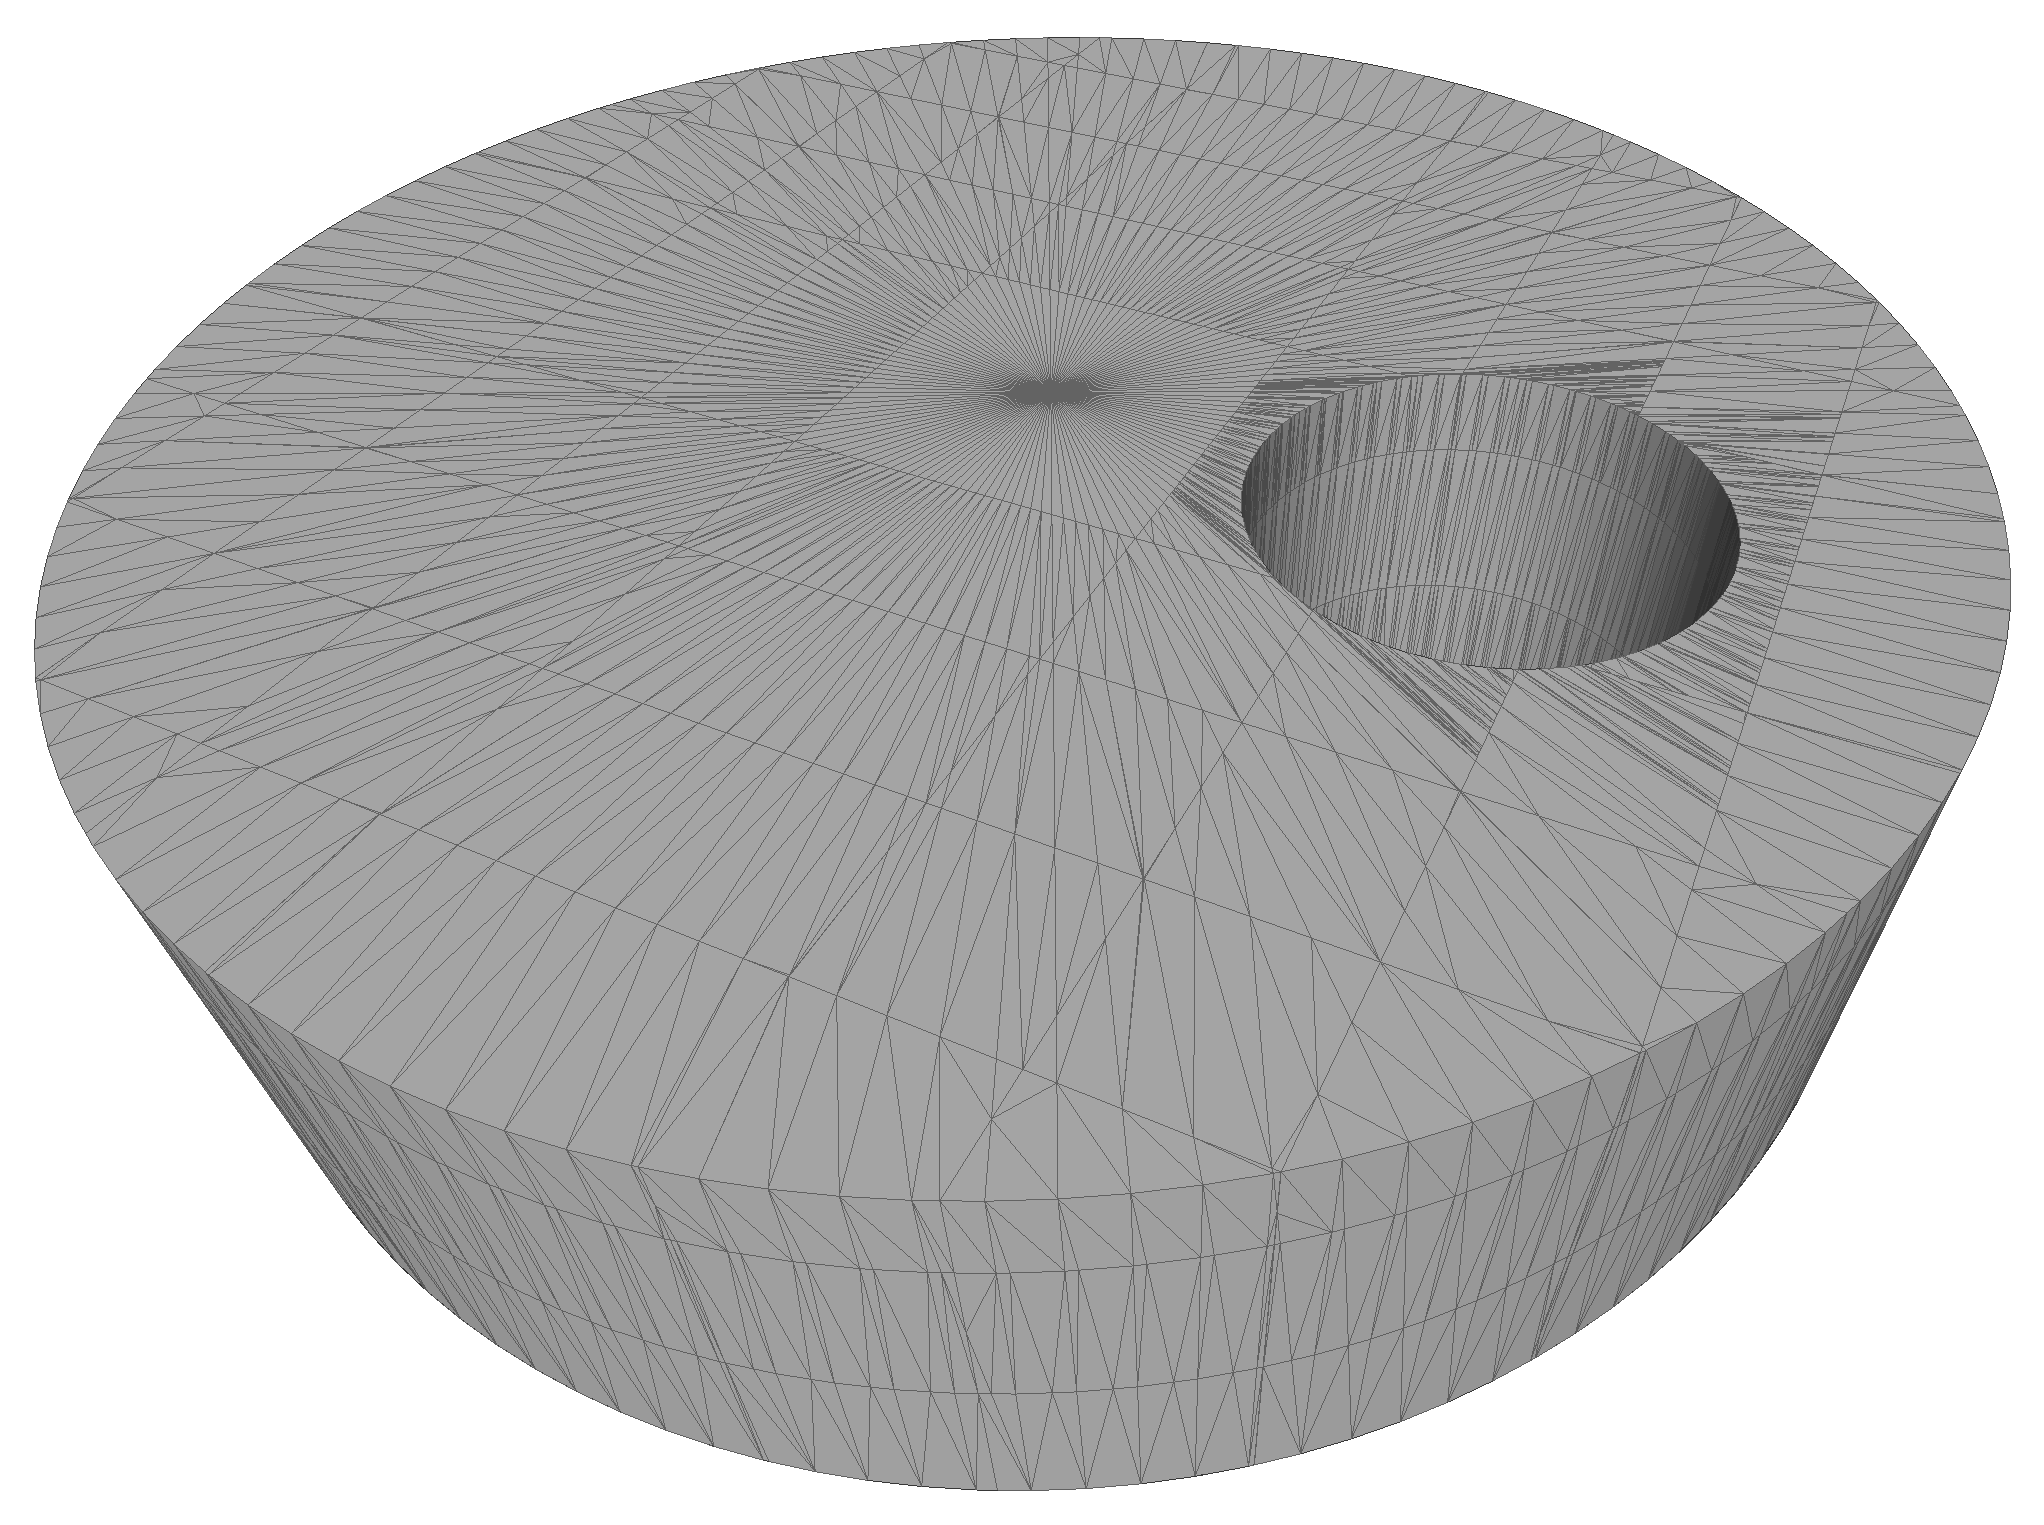
\includegraphics[width=\textwidth]{di_cylinders}
		\caption{cylinders}
		\label{fig:di_cylinders}
	\end{subfigure}
	\hspace{1cm}
	\begin{subfigure}[b]{0.34\textwidth}
		\centering
		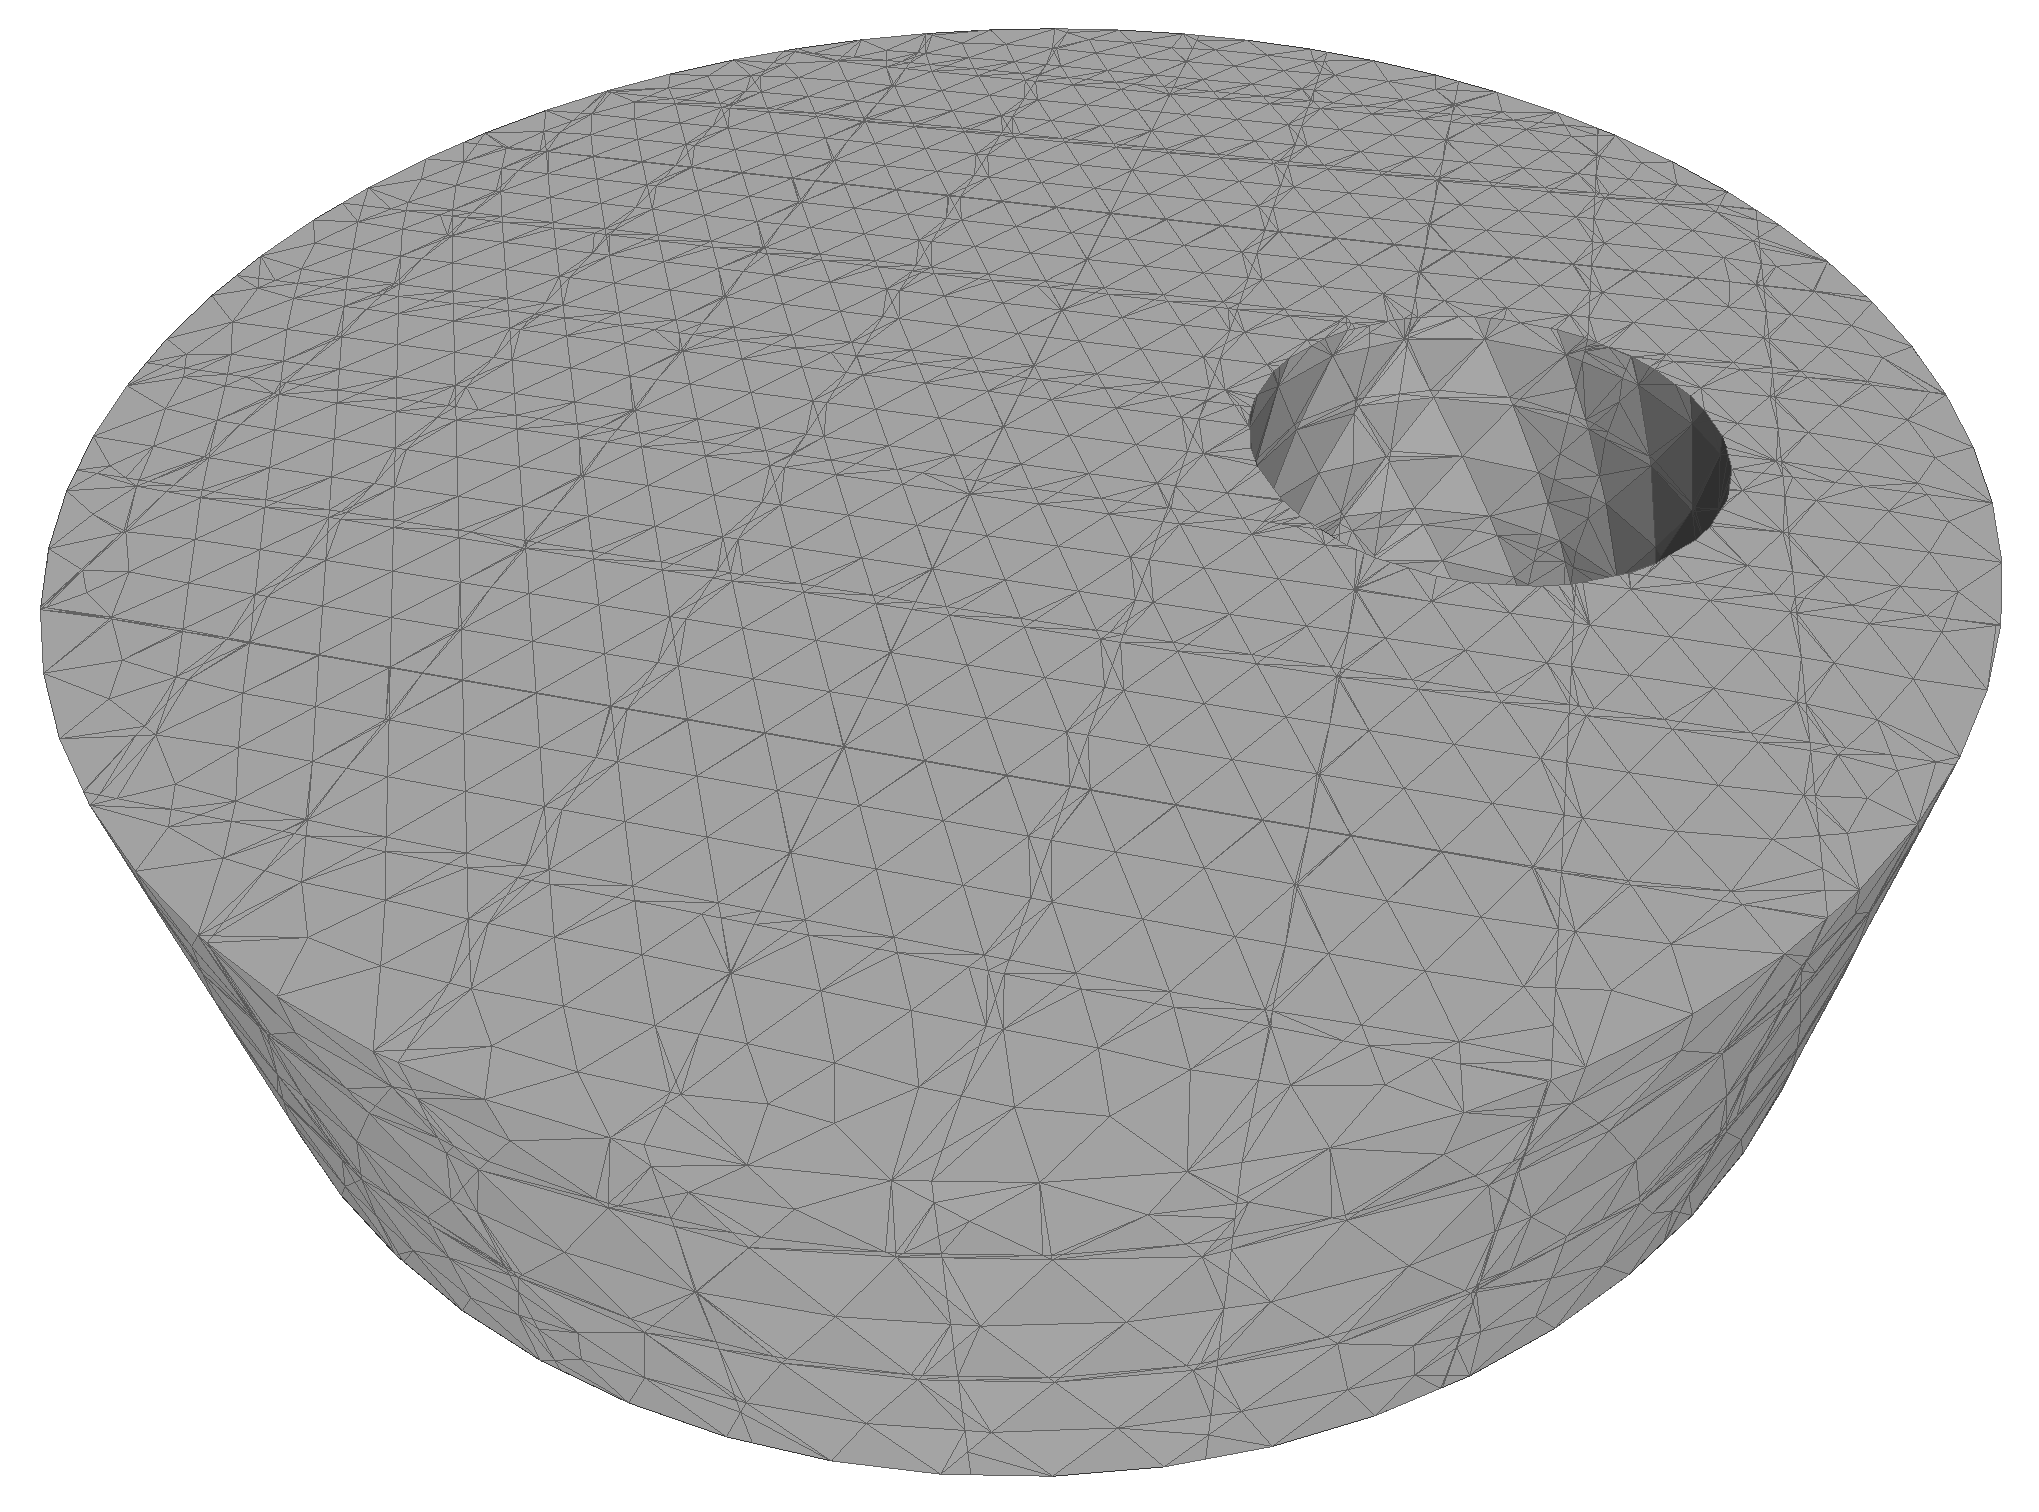
\includegraphics[width=\textwidth]{di_cylinders_delaunay}
		\caption{cylinders\_d}
		\label{fig:di_cylinders_d}
	\end{subfigure}
	\begin{subfigure}[b]{0.34\textwidth}
		\centering
		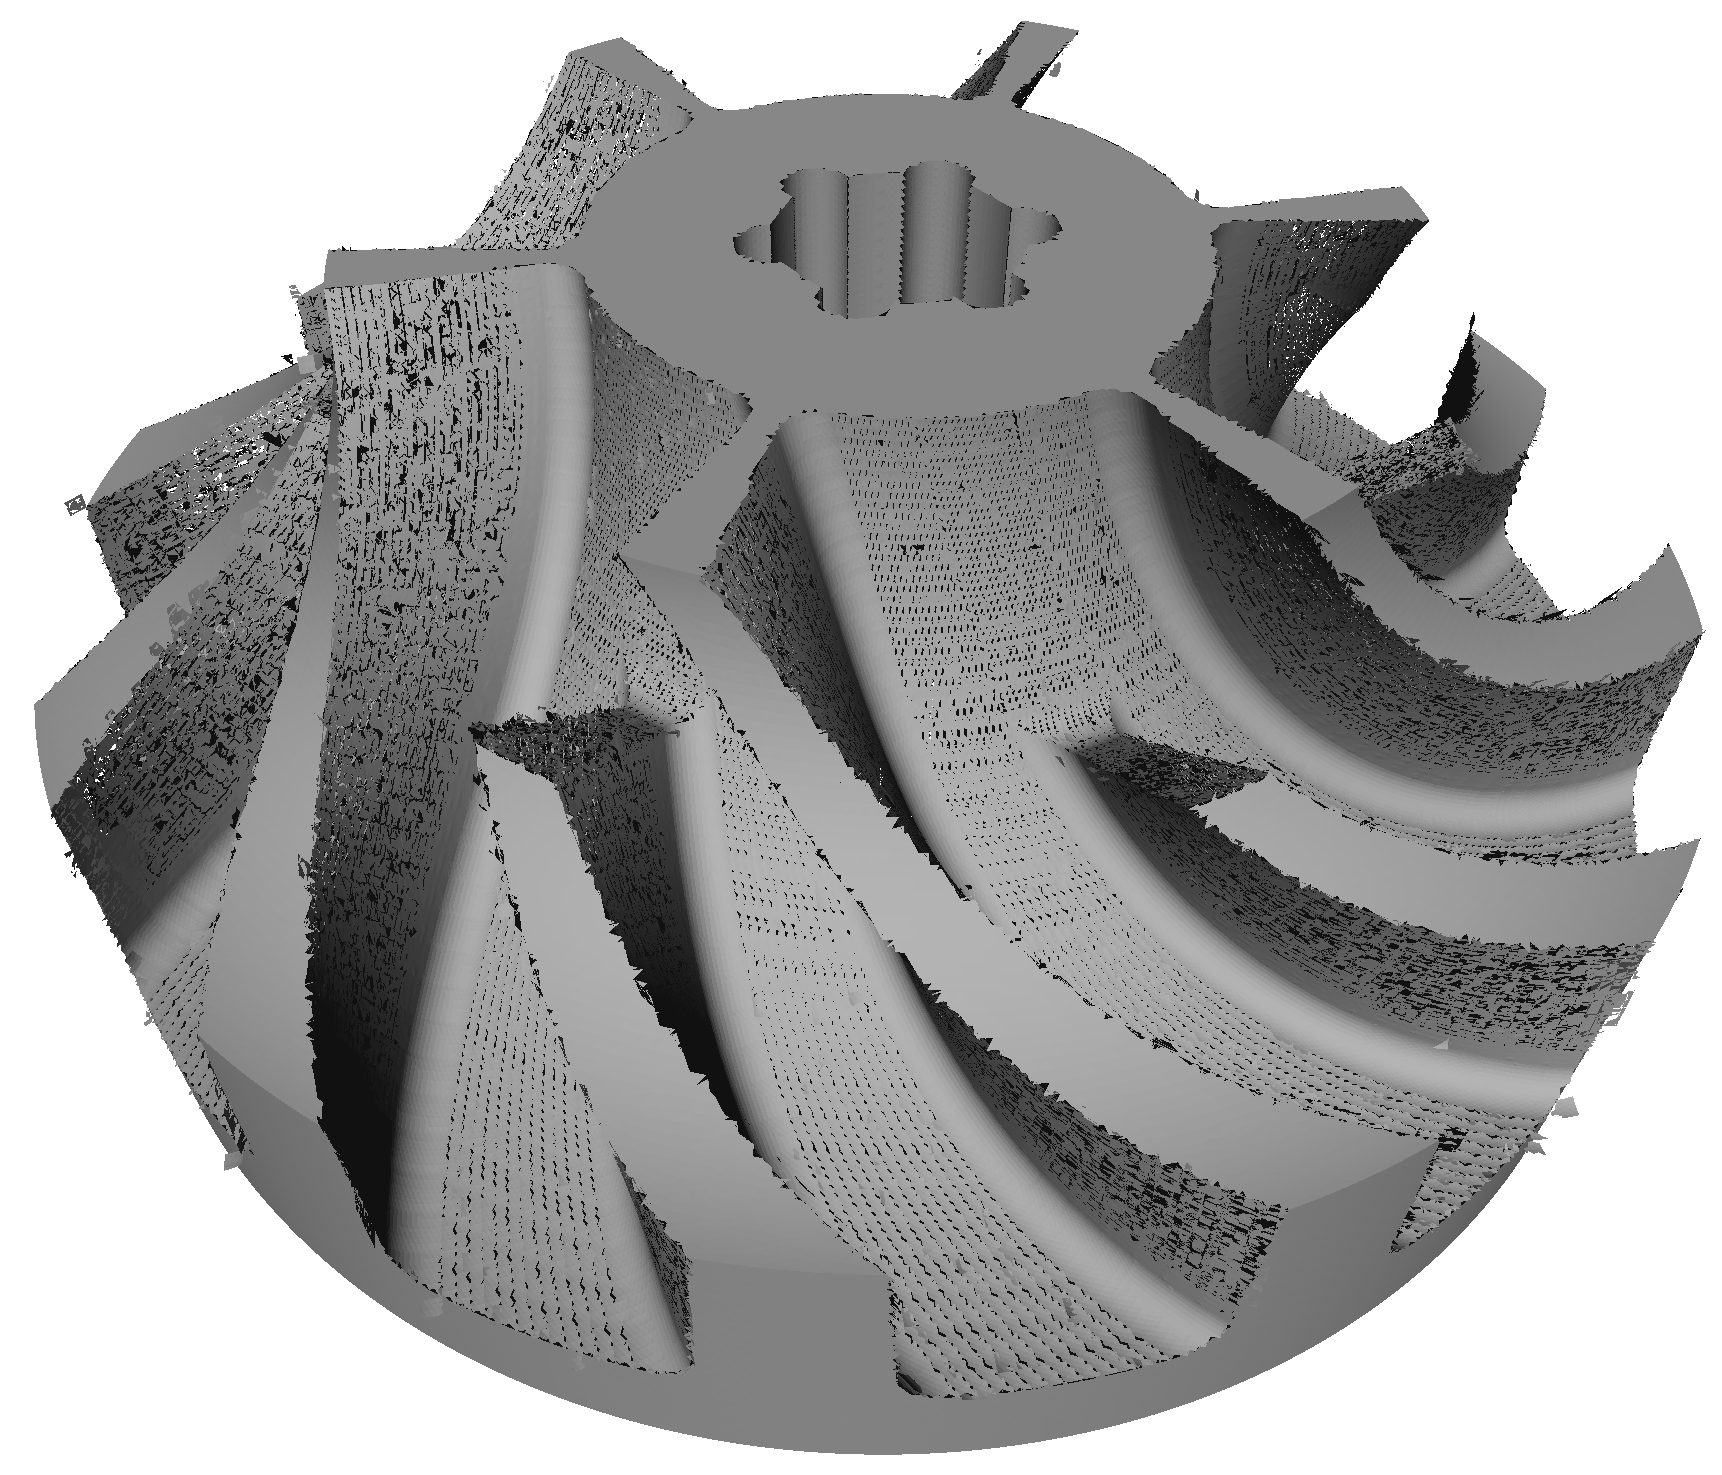
\includegraphics[width=\textwidth]{di_hq_impeller}
		\caption{impeller}
		\label{fig:di_impeller}
	\end{subfigure}
	\hspace{1cm}
	\begin{subfigure}[b]{0.34\textwidth}
		\centering
		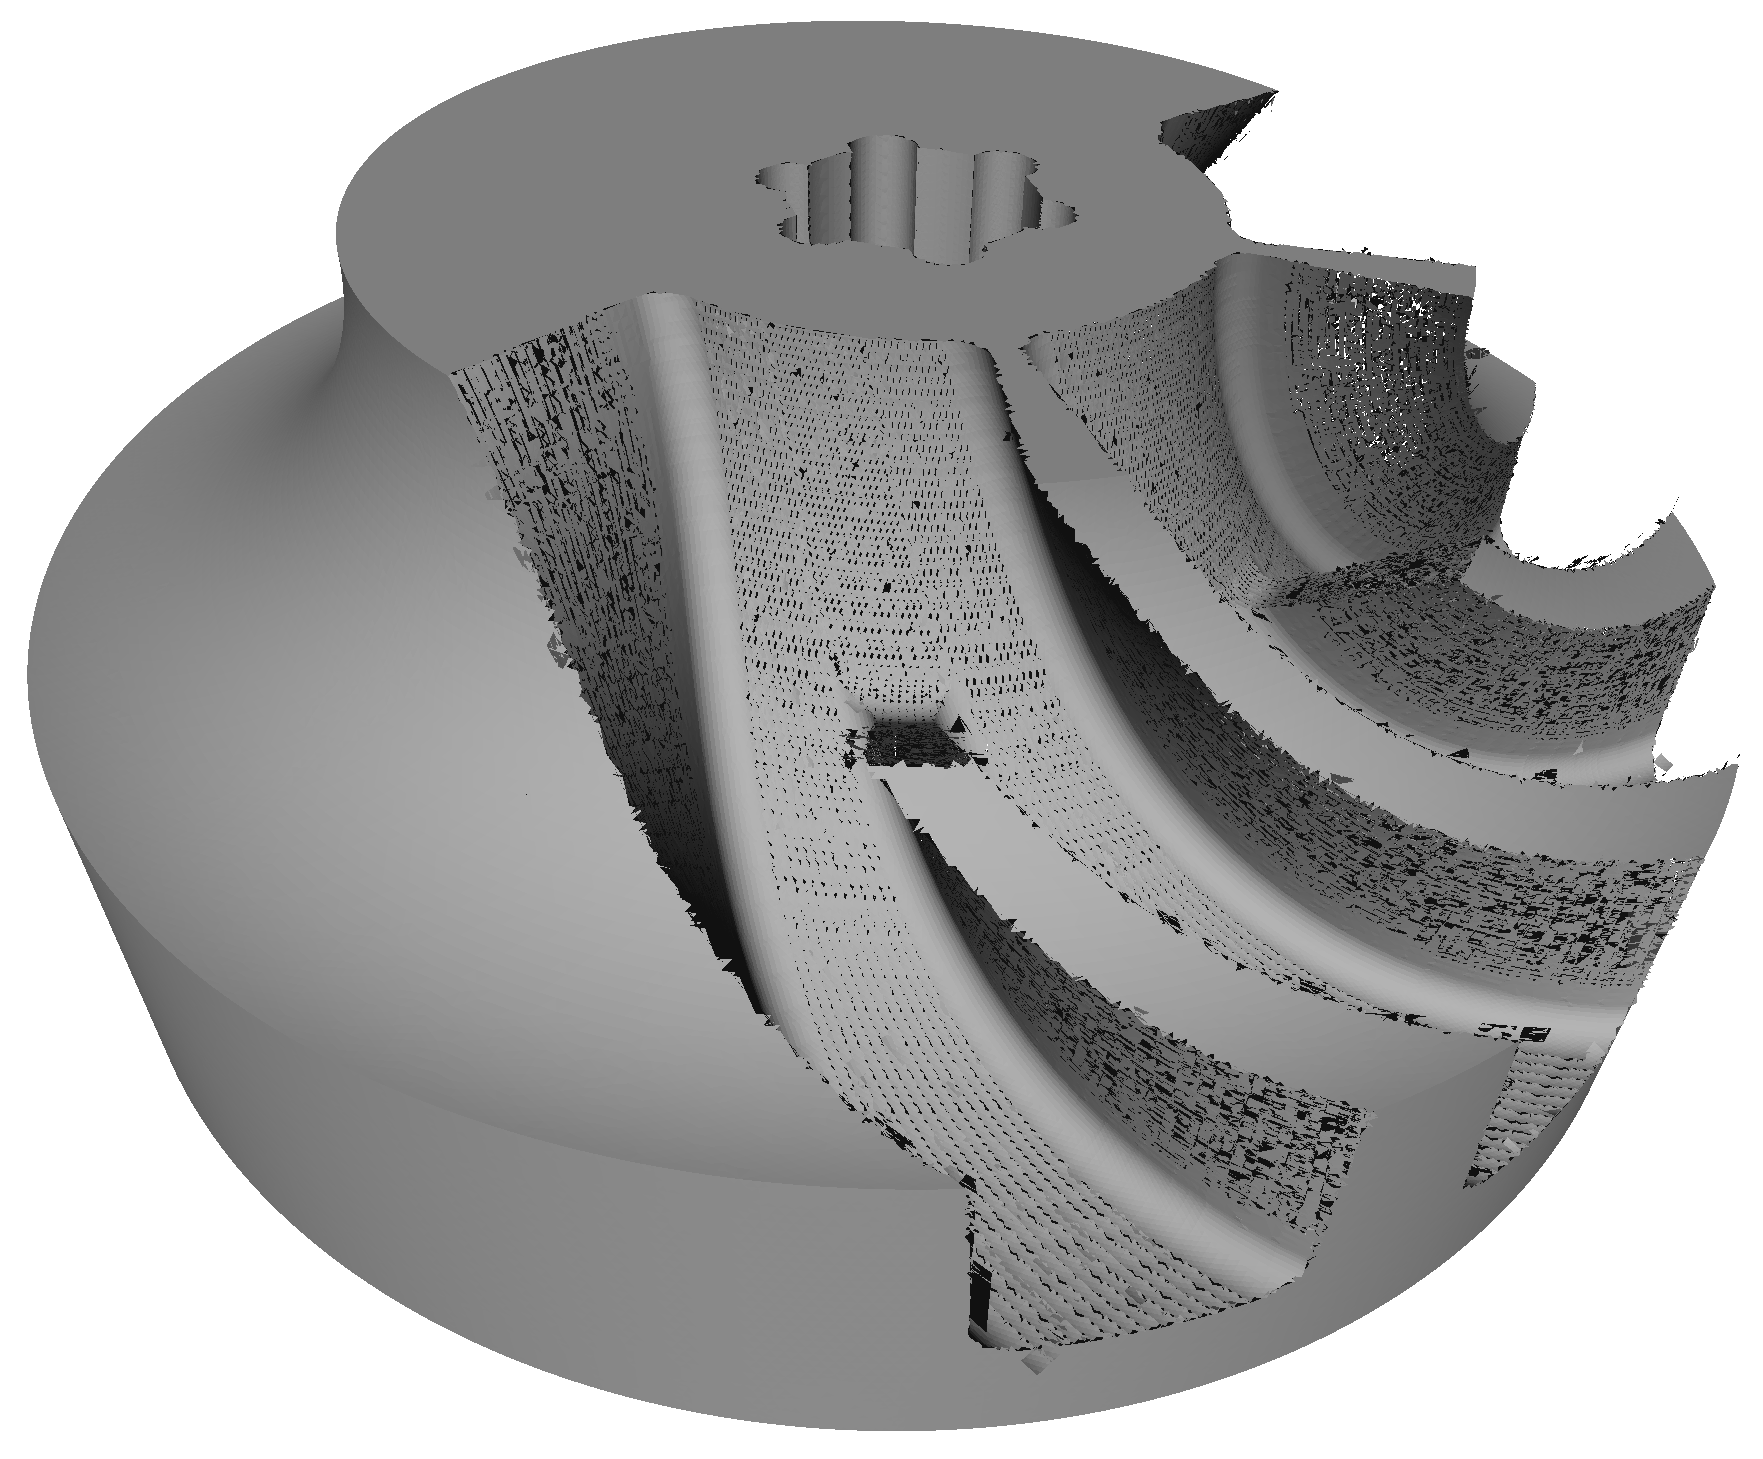
\includegraphics[width=\textwidth]{di_hq_impeller_2}
		\caption{impeller\_2}
		\label{fig:di_impeller_2}
	\end{subfigure}
	\begin{subfigure}[b]{0.33\textwidth}
		\centering
		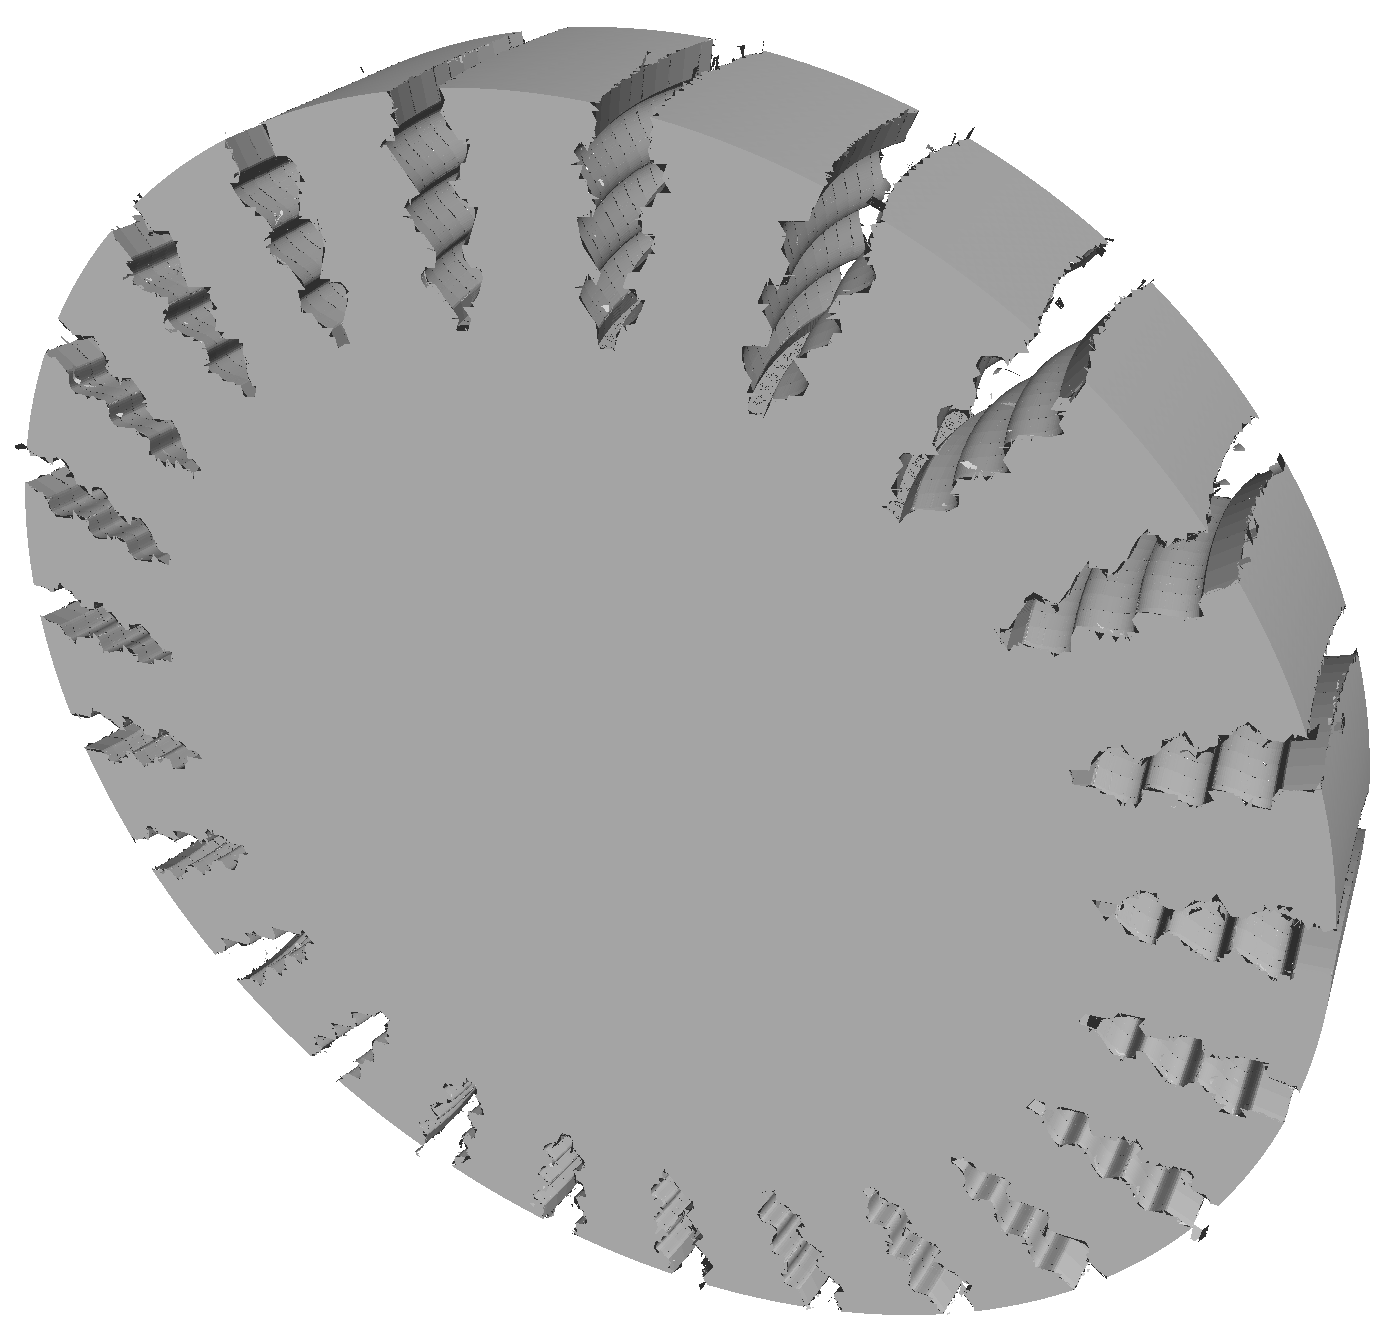
\includegraphics[width=\textwidth]{di_turbine}
		\caption{turbine}
		\label{fig:di_turbine}
	\end{subfigure}
	\caption{
		Renderings of the result meshes using MeshLab after applying the direct intersection reconstruction approach on the selected test scenes \ref{tbl:test_scenes}.
	}
	\label{fig:di_results}
\end{figure}
%
The cube2 scene has been extracted almost correctly.
All intersecting triangles have been properly split and retriangulated.
There is one small hole at one of the edges and a few falsely remaining ones at the bottom left of the cutting surface, \cf figure \ref{fig:di_cube2}.
These errors are due to a wrong outcome of the inside test, \cf \textproc{IsTriangleInsideStructure} in algorithm \ref{alg:triangle_inside_test}.
Nevertheless, the errors in the reconstructed surface are small and be corrected manually using an appropriate 3D modeling tool, creating a closed mesh.
%
Both cylinder scenes delivered good results.
The variant with the small and thin triangles even resulted in an almost perfect surface with zero holes and no leftover triangles.
Surprisingly, the other variant with the quality triangulation contained 9 holes and 1 un-eliminated triangle.
This outcome is quite the opposite of what had been observed during the development of the algorithm.
In early stages, before the GTE library had been used for its excellent CDT, the core problem was the correct splitting of intersected triangles, which was much easier on smaller and more regular triangles.
With the use of GTE, the numeric problems shifted from the CDT to the \textproc{IsTriangleInsideStructure} test.
The reason why smaller and more regular triangles entail a higher error rate in this test is not entirely clear.
The test is quite sensitive to the chosen target point of the structure used for casting the test ray.
Furthermore, a lot if ray-triangle intersections are performed where triangle normals are compared with the ray's direction, \cf details of algorithm \ref{alg:triangle_inside_test}.
All these tests become numerically unstable, if the ray becomes parallel to the tested triangles.
In theory, the tested triangle should always lie clearly inside or outside the structure it is tested against, otherwise there must have been an intersection and the triangle would have been split.
In practice, if an intersection has been missed and the triangle spans the structure or the tested triangle is almost degenerated and very close to the structure, errors may occur.
%
Concerning the more complex scenes, the impeller and turbine surfaces look quite good from a distance, but fail horribly reviewing the details.
Figure \ref{fig:di_scenes_artifacts} shows two detailed views, one centered on a smaller blade of the impeller and one centered on a milling groove of the turbine.
%
\begin{figure}[h]
	\centering
	\begin{subfigure}[b]{\textwidth}
		\centering
		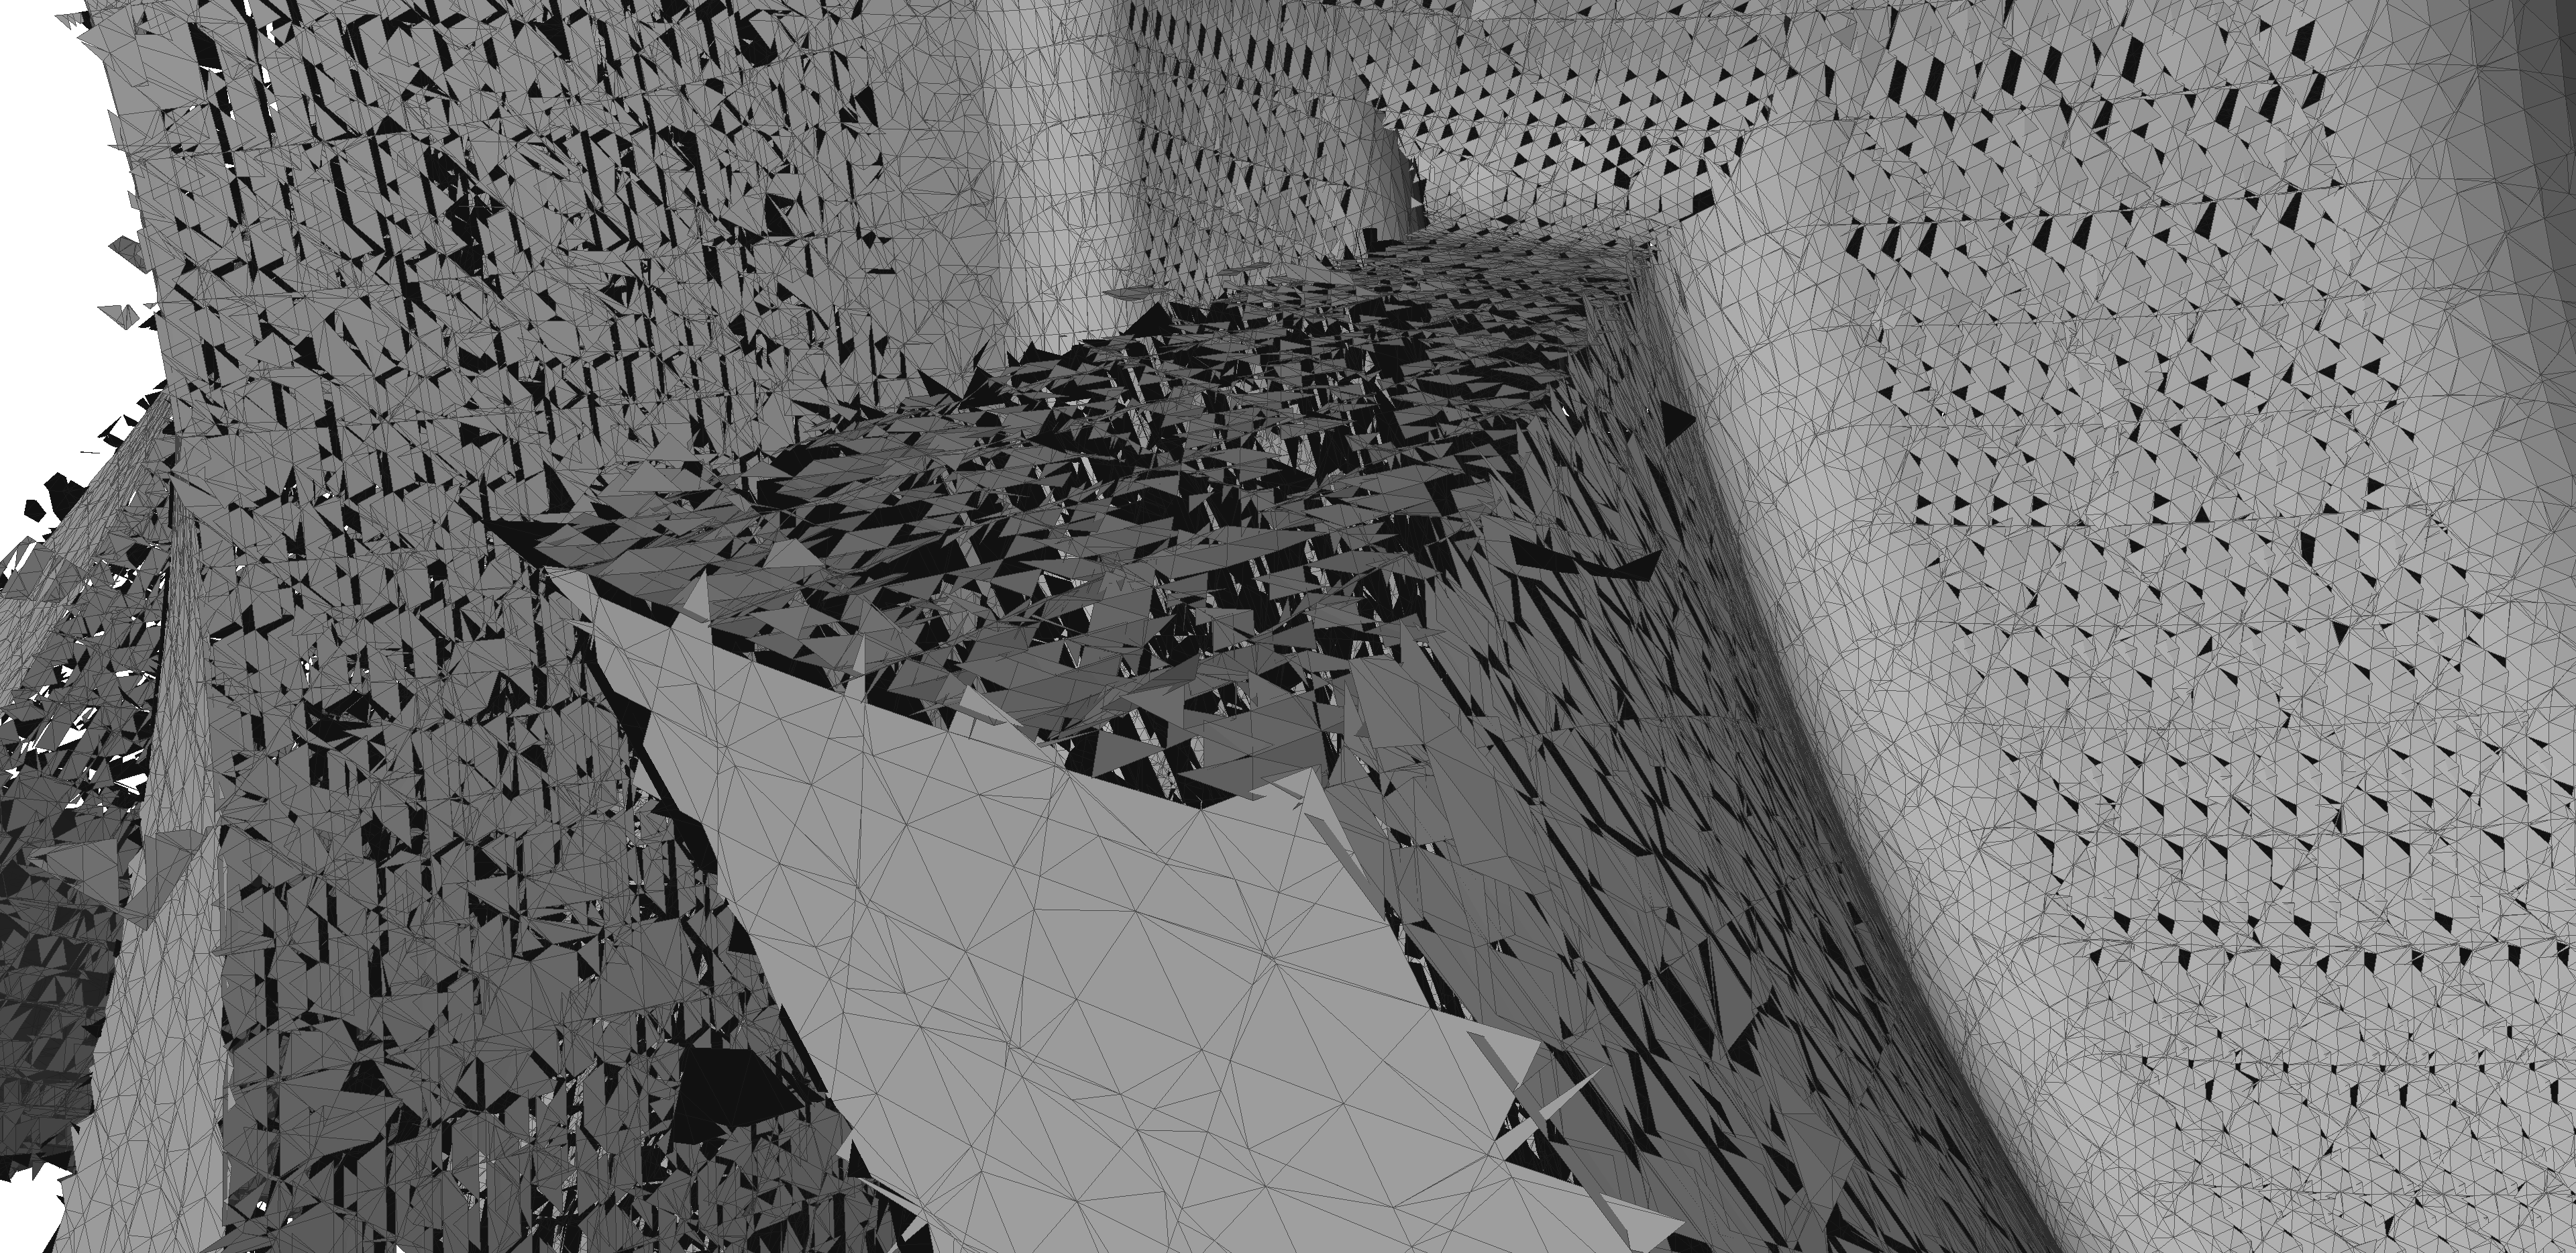
\includegraphics[width=0.8\textwidth]{di_hq_impeller_detail}
		\caption{impeller}
		\label{fig:di_impeller_detail}
	\end{subfigure}\\
	\begin{subfigure}[b]{\textwidth}
		\centering
		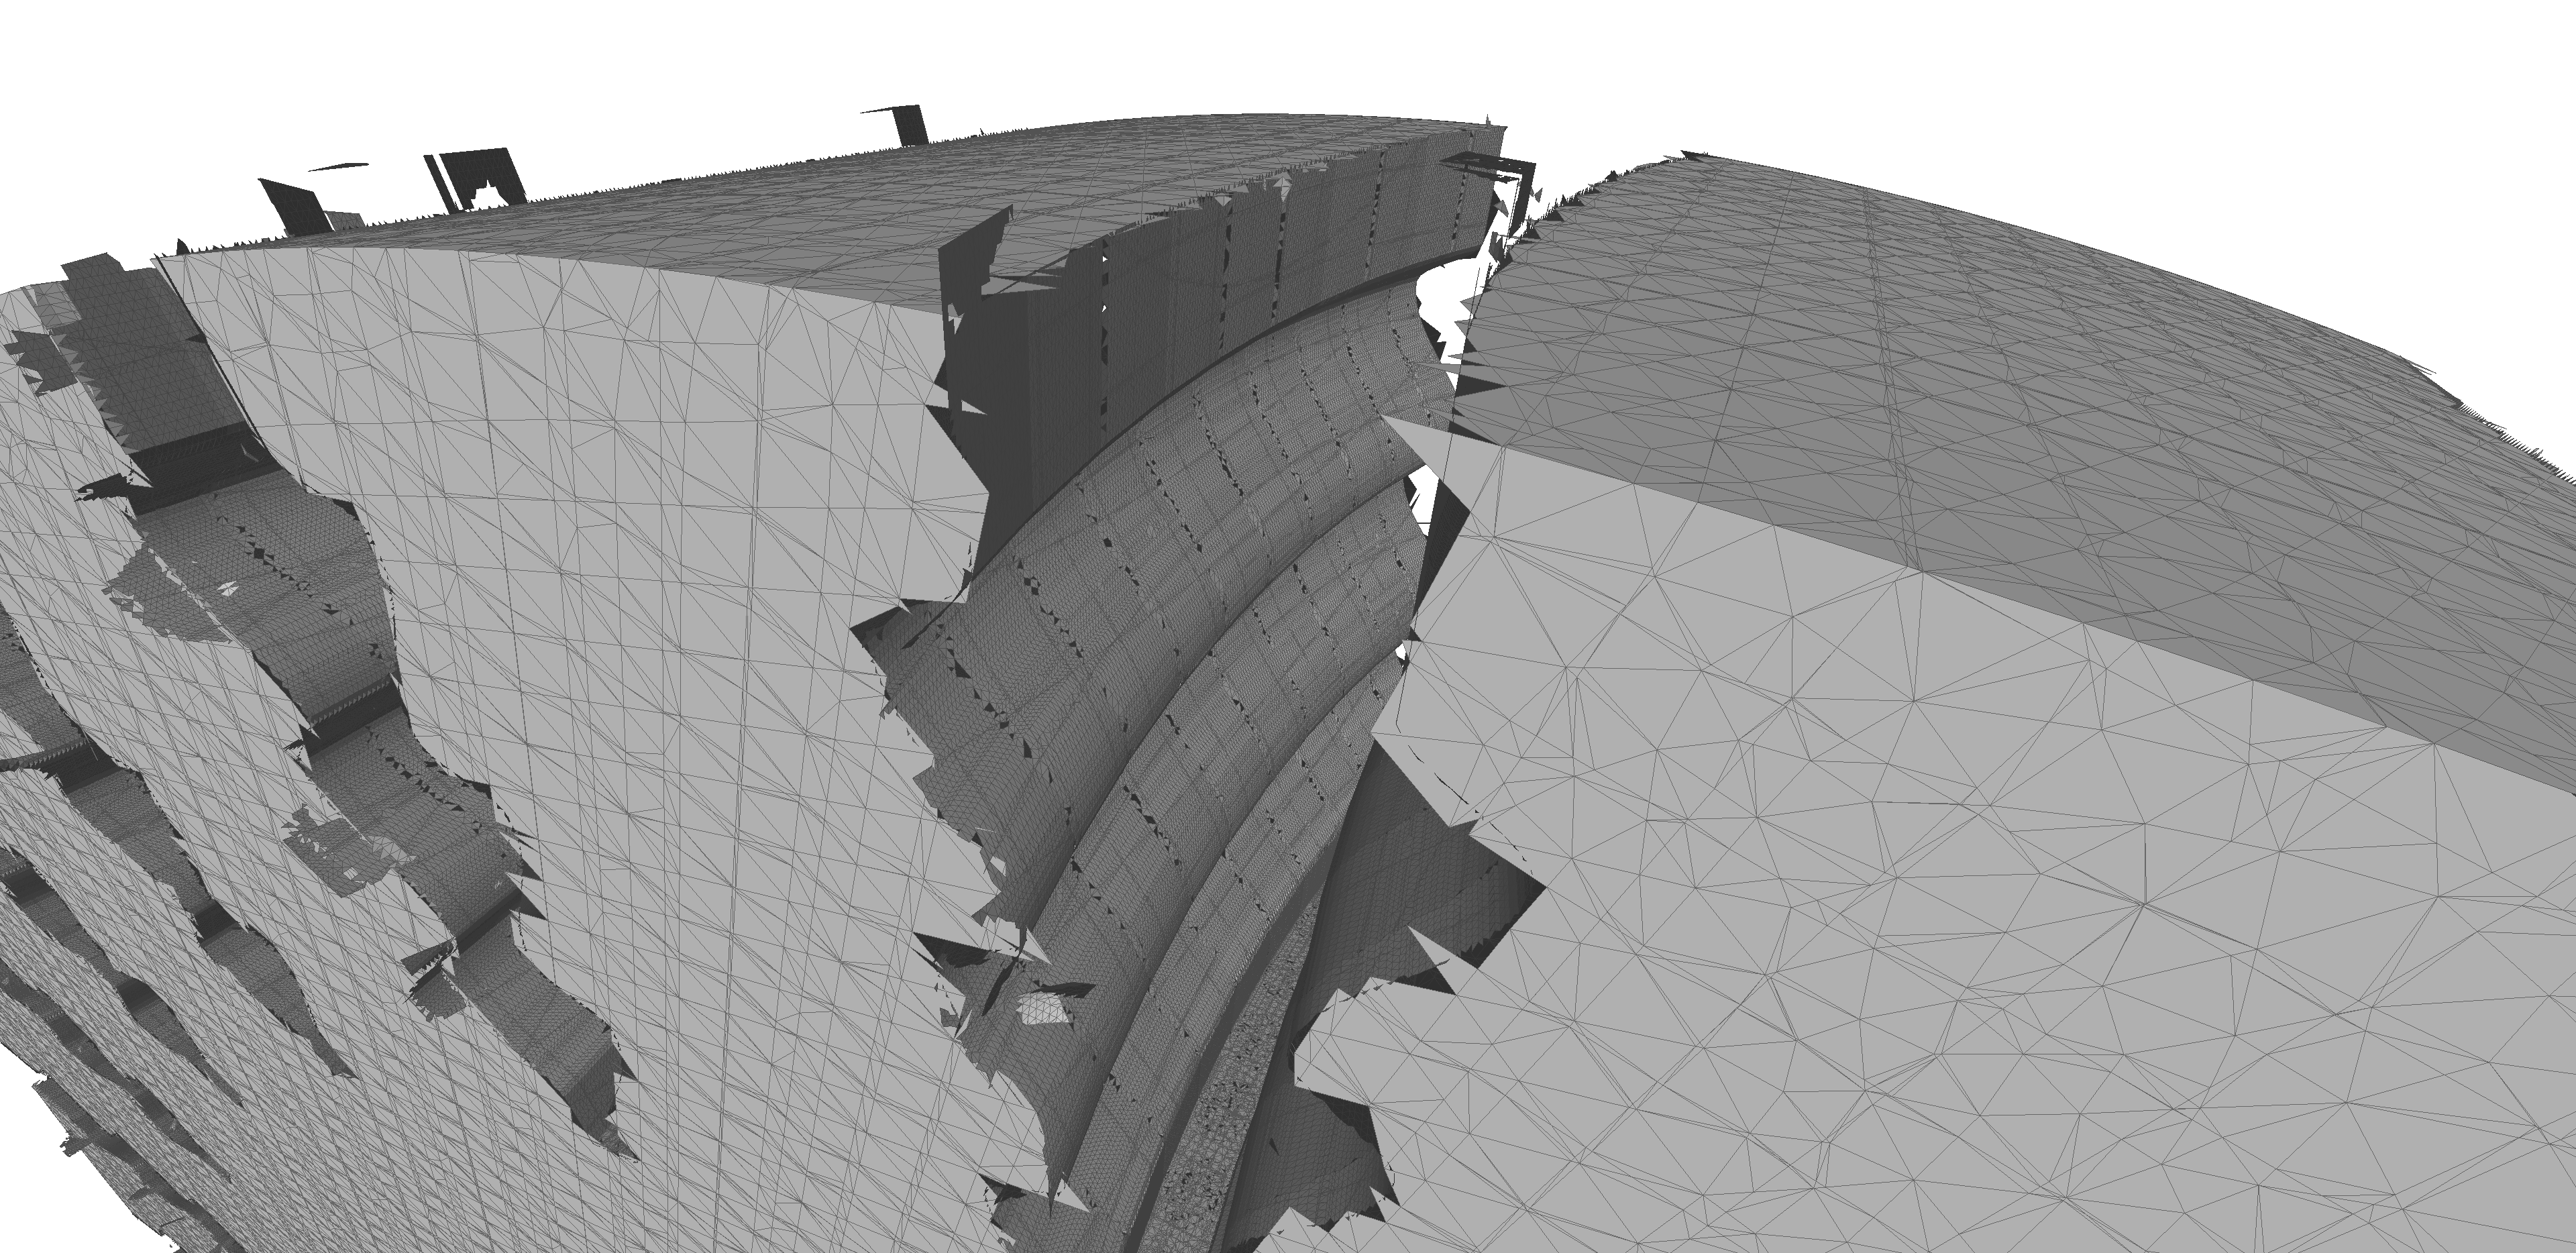
\includegraphics[width=0.8\textwidth]{di_turbine_detail}
		\caption{turbine}
		\label{fig:di_turbine_detail}
	\end{subfigure}
	\caption{
		Renderings of details of the impeller and turbine scene result meshes using MeshLab after applying the direct intersection reconstruction approach.
	}
	\label{fig:di_scenes_artifacts}
\end{figure}
%
Especially the impeller scene contains quite a lot of intersecting triangles and structures in each cell.
When zooming very close to the edges of a blade, several intersecting triangles can be seen which have not been split, probably due to errors when detecting the intersection lines.
These errors may then cause consequential errors in \eg the triangle inside test.
As the impeller's grid contains cells with up to 64 structures, small mistakes add up iteratively and may cause huge defects on the final surface.
Especially the cells which contain triangles from many swept volumes, \ie cells at the blade edges, suffer from this effect.
The triangle inside test still does an acceptable job and the final surface does somehow resemble the surface.
Nonetheless, the reconstructed surface contains a huge number of holes and boundaries as well as lots of intersecting triangles.
Regarding the quality of the produces mesh, the result is probably worthless for subsequent tasks, like using it for simulations.
%
The turbine scene seems to have a similar problem.
Most of the intersections between stock and swept volume triangles have not been caught.
As the total number of swept volumes is relatively low compared to the impeller scene and only very few of them intersect each other, the surface errors are considerably smaller.
By deleting self intersecting triangles from the outcome, an intelligent hole closing algorithm might be able to recover a closed surface, \eg an adaption of the ball-pivoting algorithm. %TODO cite BPA close boundary loops.

All extracted meshes in general have issues with neighboring triangles not having identical shared vertices.
The difference however is neglectable and can easily be corrected in a post processing step which merges close vertices, \eg using the Merge Close Vertices filter of MeshLab.
Furthermore, the result contains many T-vertices around intersected triangles which result from clipping a cell's triangles after the triangle-triangle intersections and retriangulations instead of before, \cf section \ref{sec:clipping}.
